\documentclass[10pt]{article}
\usepackage[utf8]{inputenc}
\usepackage[T1]{fontenc}
\usepackage{amsmath}
\usepackage{amsfonts}
\usepackage{amssymb}
\usepackage[version=4]{mhchem}
\usepackage{stmaryrd}
\usepackage{graphicx}
\usepackage[export]{adjustbox}
\graphicspath{ {./images/} }

\title{2023학년도 대학수학능력시험 문제지 }

\author{}
\date{}


\begin{document}
\maketitle
제 2 교시

\section{수학 영역}
홀수형

\section{5 지선다형}
\begin{enumerate}
  \item $\left(\frac{4}{2^{\sqrt{2}}}\right)^{2+\sqrt{2}}$ 의 값은? [2점]
(1) $\frac{1}{4}$
(2) $\frac{1}{2}$
(3) 1
(4) 2
(5) 4

  \item $\lim _{x \rightarrow \infty} \frac{\sqrt{x^{2}-2}+3 x}{x+5}$ 의 값은? [2점]
(1) 1
(2) 2
(3) 3
(4) 4
(5) 5

  \item 공비가 양수인 등비수열 $\left\{a_{n}\right\}$ 이

\end{enumerate}

$$
a_{2}+a_{4}=30, \quad a_{4}+a_{6}=\frac{15}{2}
$$

를 만족시킬 때, $a_{1}$ 의 값은? [3점]
(1) 48
(2) 56
(3) 64
(4) 72
(5) 80

\begin{enumerate}
  \setcounter{enumi}{3}
  \item 다항함수 $f(x)$ 에 대하여 함수 $g(x)$ 를
\end{enumerate}

$$
g(x)=x^{2} f(x)
$$

라 하자. $f(2)=1, f^{\prime}(2)=3$ 일 때, $g^{\prime}(2)$ 의 값은? [3점]
(1) 12
(2) 14
(3) 16
(4) 18
(5) 20 5. $\tan \theta<0$ 이고 $\cos \left(\frac{\pi}{2}+\theta\right)=\frac{\sqrt{5}}{5}$ 일 때, $\cos \theta$ 의 값은? [3점]
(1) $-\frac{2 \sqrt{5}}{5}$
(2) $-\frac{\sqrt{5}}{5}$
(3) 0
(4) $\frac{\sqrt{5}}{5}$
(5) $\frac{2 \sqrt{5}}{5}$

\begin{enumerate}
  \setcounter{enumi}{5}
  \item 함수 $f(x)=2 x^{3}-9 x^{2}+a x+5$ 는 $x=1$ 에서 극대이고, $x=b$ 에서 극소이다. $a+b$ 의 값은? (단, $a, b$ 는 상수이다.) [3점]
(1) 12
(2) 14
(3) 16
(4) 18
(5) 20

  \item 모든 항이 양수이고 첫째항과 공차가 같은 등차수열 $\left\{a_{n}\right\}$ 이

\end{enumerate}

$$
\sum_{k=1}^{15} \frac{1}{\sqrt{a_{k}}+\sqrt{a_{k+1}}}=2
$$

를 만족시킬 때, $a_{4}$ 의 값은? [3점]
(1) 6
(2) 7
(3) 8
(4) 9
(5) 10 8. 점 $(0,4)$ 에서 곡선 $y=x^{3}-x+2$ 에 그은 접선의 $x$ 절편은? [3점]
(1) $-\frac{1}{2}$
(2) -1
(3) $-\frac{3}{2}$
(4) -2
(5) $-\frac{5}{2}$

\begin{enumerate}
  \setcounter{enumi}{8}
  \item 함수
\end{enumerate}

$$
f(x)=a-\sqrt{3} \tan 2 x
$$

가 닫힌구간 $\left[-\frac{\pi}{6}, b\right]$ 에서 최댓값 7 , 최솟값 3 을 가질 때, $a \times b$ 의 값은? (단, $a, b$ 는 상수이다.) [4점]
(1) $\frac{\pi}{2}$
(2) $\frac{5 \pi}{12}$
(3) $\frac{\pi}{3}$
(4) $\frac{\pi}{4}$
(5) $\frac{\pi}{6}$

\begin{enumerate}
  \setcounter{enumi}{9}
  \item 두 곡선 $y=x^{3}+x^{2}, y=-x^{2}+k$ 와 $y$ 축으로 둘러싸인 부분의 넓이를 $A$, 두 곡선 $y=x^{3}+x^{2}, y=-x^{2}+k$ 와 직선 $x=2$ 로 둘러싸인 부분의 넓이를 $B$ 라 하자. $A=B$ 일 때, 상수 $k$ 의 값은? (단, $4<k<5$ ) [4점]
(1) $\frac{25}{6}$
(2) $\frac{13}{3}$
(3) $\frac{9}{2}$
(4) $\frac{14}{3}$
(5) $\frac{29}{6}$
\end{enumerate}

\begin{center}
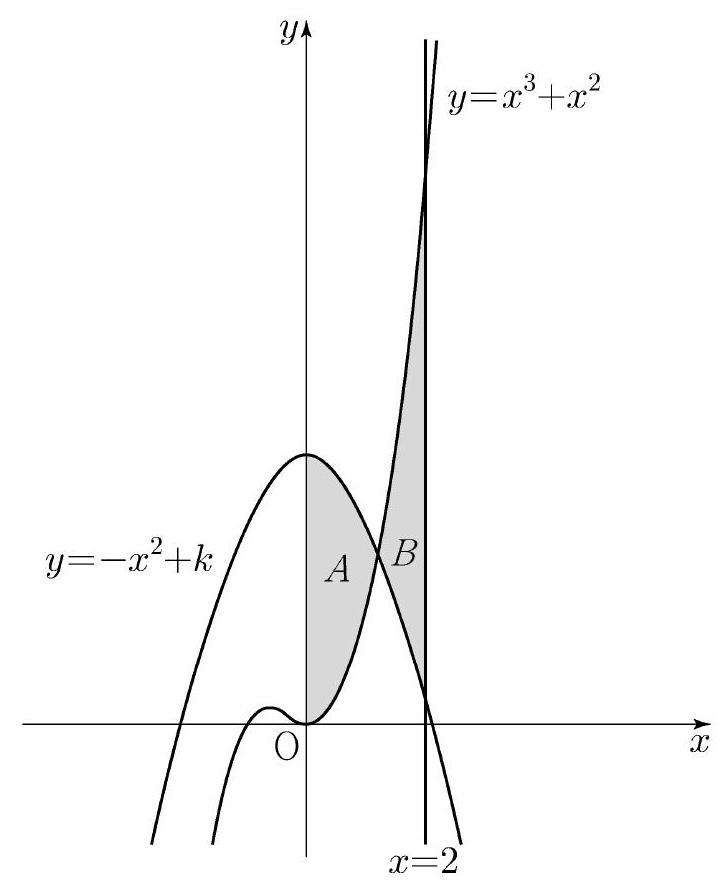
\includegraphics[max width=\textwidth]{2023_06_06_b380aa8523ec7afae994g-03}
\end{center}

\begin{enumerate}
  \setcounter{enumi}{10}
  \item 그림과 같이 사각형 $\mathrm{ABCD}$ 가 한 원에 내접하고
\end{enumerate}

$$
\overline{\mathrm{AB}}=5, \overline{\mathrm{AC}}=3 \sqrt{5}, \overline{\mathrm{AD}}=7, \angle \mathrm{BAC}=\angle \mathrm{CAD}
$$

일 때, 이 원의 반지름의 길이는? [4점]

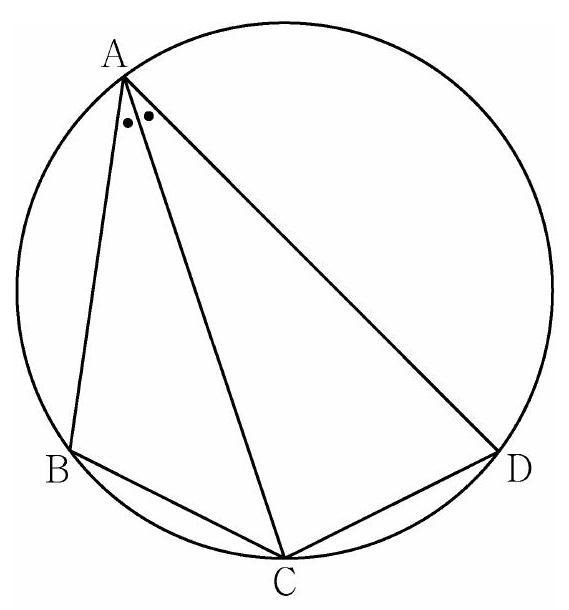
\includegraphics[max width=\textwidth, center]{2023_06_06_b380aa8523ec7afae994g-04}
(1) $\frac{5 \sqrt{2}}{2}$
(2) $\frac{8 \sqrt{5}}{5}$
(3) $\frac{5 \sqrt{5}}{3}$
(4) $\frac{8 \sqrt{2}}{3}$
(5) $\frac{9 \sqrt{3}}{4}$

\begin{enumerate}
  \setcounter{enumi}{11}
  \item 실수 전체의 집합에서 연속인 함수 $f(x)$ 가 다음 조건을 만족시킨다.
\end{enumerate}

$n-1 \leq x<n$ 일 때, $|f(x)|=|6(x-n+1)(x-n)|$ 이다. (단, $n$ 은 자연수이다.)

열린구간 $(0,4)$ 에서 정의된 함수

$$
g(x)=\int_{0}^{x} f(t) d t-\int_{x}^{4} f(t) d t
$$

가 $x=2$ 에서 최솟값 0 을 가질 때, $\int_{\frac{1}{2}}^{4} f(x) d x$ 의 값은? [4점]
(1) $-\frac{3}{2}$
(2) $-\frac{1}{2}$
(3) $\frac{1}{2}$
(4) $\frac{3}{2}$
(5) $\frac{5}{2}$ 13. 자연수 $m(m \geq 2)$ 에 대하여 $m^{12}$ 의 $n$ 제곱근 중에서 정수가 존재하도록 하는 2 이상의 자연수 $n$ 의 개수를 $f(m)$ 이라 할 때, $\sum_{m=2}^{9} f(m)$ 의 값은? [4점]
(1) 37
(2) 42
(3) 47
(4) 52
(5) 57

\begin{enumerate}
  \setcounter{enumi}{13}
  \item 다항함수 $f(x)$ 에 대하여 함수 $g(x)$ 를 다음과 같이 정의한다.
\end{enumerate}

$$
g(x)= \begin{cases}x & (x<-1 \text { 또는 } x>1) \\ f(x) & (-1 \leq x \leq 1)\end{cases}
$$

함수 $h(x)=\lim _{t \rightarrow 0+} g(x+t) \times \lim _{t \rightarrow 2+} g(x+t)$ 에 대하여

<보기>에서 옳은 것만을 있는 대로 고른 것은? [4점]

ᄀ. $h(1)=3$

ㄴ. 함수 $h(x)$ 는 실수 전체의 집합에서 연속이다.

ㄷ. 함수 $g(x)$ 가 닫힌구간 $[-1,1]$ 에서 감소하고 $g(-1)=-2$ 이면 함수 $h(x)$ 는 실수 전체의 집합에서 최솟값을 갖는다.
(1) ᄀ
(2) 1
(3) ᄀ, ᄂ (4) ᄀ, ᄃ
(5) ᄂ, ᄃ 15. 모든 항이 자연수이고 다음 조건을 만족시키는 모든 수열 $\left\{a_{n}\right\}$ 에 대하여 $a_{9}$ 의 최댓값과 최솟값을 각각 $M, m$ 이라 할 때, $M+m$ 의 값은? [4점]

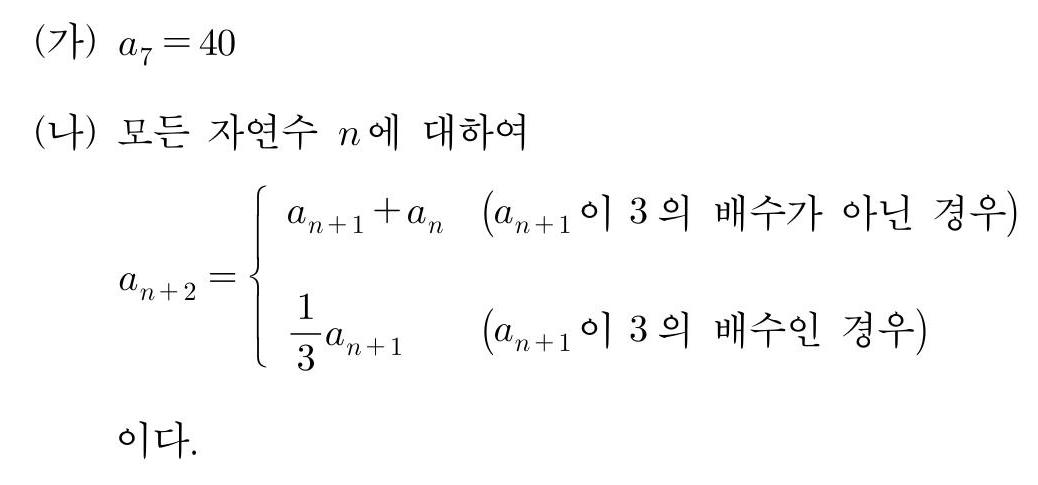
\includegraphics[max width=\textwidth, center]{2023_06_06_b380aa8523ec7afae994g-06}
(1) 216
(2) 218
(3) 220
(4) 222
(5) 224

\section{단답형}
\begin{enumerate}
  \setcounter{enumi}{15}
  \item 방정식
\end{enumerate}

$$
\log _{2}(3 x+2)=2+\log _{2}(x-2)
$$

를 만족시키는 실수 $x$ 의 값을 구하시오. [3점]

\begin{enumerate}
  \setcounter{enumi}{16}
  \item 함수 $f(x)$ 에 대하여 $f^{\prime}(x)=4 x^{3}-2 x$ 이고 $f(0)=3$ 일 때, $f(2)$ 의 값을 구하시오. [3점] 18. 두 수열 $\left\{a_{n}\right\},\left\{b_{n}\right\}$ 에 대하여
\end{enumerate}

$$
\sum_{k=1}^{5}\left(3 a_{k}+5\right)=55, \quad \sum_{k=1}^{5}\left(a_{k}+b_{k}\right)=32
$$

일 때, $\sum_{k=1}^{5} b_{k}$ 의 값을 구하시오. [3점]

\begin{enumerate}
  \setcounter{enumi}{18}
  \item 방정식 $2 x^{3}-6 x^{2}+k=0$ 의 서로 다른 양의 실근의 개수가 2 가 되도록 하는 정수 $k$ 의 개수를 구하시오. [3점] 20. 수직선 위를 움직이는 점 $\mathrm{P}$ 의 시각 $t(t \geq 0)$ 에서의 속도 $v(t)$ 와 가속도 $a(t)$ 가 다음 조건을 만족시킨다.
\end{enumerate}

(가) $0 \leq t \leq 2$ 일 때, $v(t)=2 t^{3}-8 t$ 이다.

(나) $t \geq 2$ 일 때, $a(t)=6 t+4$ 이다.

시각 $t=0$ 에서 $t=3$ 까지 점 $\mathrm{P}$ 가 움직인 거리를 구하시오. [4점] 21. 자연수 $n$ 에 대하여 함수 $f(x)$ 를

$$
f(x)= \begin{cases}\left|3^{x+2}-n\right| & (x<0) \\ \left|\log _{2}(x+4)-n\right| & (x \geq 0)\end{cases}
$$

이라 하자. 실수 $t$ 에 대하여 $x$ 에 대한 방정식 $f(x)=t$ 의 서로 다른 실근의 개수를 $g(t)$ 라 할 때, 함수 $g(t)$ 의 최댓값이 4 가 되도록 하는 모든 자연수 $n$ 의 값의 합을 구하시오. [4점] 22. 최고차항의 계수가 1 인 삼차함수 $f(x)$ 와 실수 전체의 집합에서 연속인 함수 $g(x)$ 가 다음 조건을 만족시킬 때, $f(4)$ 의 값을 구하시오. [4점]

(가) 모든 실수 $x$ 에 대하여

$$
f(x)=f(1)+(x-1) f^{\prime}(g(x)) \text { 이다. }
$$

(나) 함수 $g(x)$ 의 최솟값은 $\frac{5}{2}$ 이다.

(다) $f(0)=-3, f(g(1))=6$

\section{* 확인 사항}
○ 답안지의 해당란에 필요한 내용을 정확히 기입(표기)했는지 확인 하시오.

○ 이어서, 「선택과목(확률과 통계)」 문제가 제시되오니, 자신이 선택한 과목인지 확인하시오.

\section{3학년도 대학수학능력시험 문제지
제2교시 수학 영역(확률과 통계)
홀수형}
5 지선다형

\begin{enumerate}
  \setcounter{enumi}{22}
  \item 다항식 $\left(x^{3}+3\right)^{5}$ 의 전개식에서 $x^{9}$ 의 계수는? [2점]
(1) 30
(2) 60
(3) 90
(4) 120
(5) 150

  \item 숫자 $1,2,3,4,5$ 중에서 중복을 허락하여 4 개를 택해 일렬로 나열하여 만들 수 있는 네 자리의 자연수 중 4000 이상인 홀수의 개수는? [3점]
(1) 125
(2) 150
(3) 175
(4) 200
(5) 225 25. 흰색 마스크 5 개, 검은색 마스크 9 개가 들어 있는 상자가 있다. 이 상자에서 임의로 3 개의 마스크를 동시에 꺼낼 때, 꺼낸 3 개의 마스크 중에서 적어도 한 개가 흰색 마스크일 확률은? [3점]
(1) $\frac{8}{13}$
(2) $\frac{17}{26}$
(3) $\frac{9}{13}$
(4) $\frac{19}{26}$
(5) $\frac{10}{13}$

  \item 주머니에 1 이 적힌 흰 공 1 개, 2 가 적힌 흰 공 1 개, 1 이 적힌 검은 공 1 개, 2 가 적힌 검은 공 3 개가 들어 있다. 이 주머니에서 임의로 3 개의 공을 동시에 꺼내는 시행을 한다. 이 시행에서 꺼낸 3 개의 공 중에서 흰 공이 1 개이고 검은 공이 2 개인 사건을 $A$, 꺼낸 3 개의 공에 적혀 있는 수를 모두 곱한 값이 8 인 사건을 $B$ 라 할 때, $\mathrm{P}(A \cup B)$ 의 값은? [3점]
(1) $\frac{11}{20}$
(2) $\frac{3}{5}$
(3) $\frac{13}{20}$
(4) $\frac{7}{10}$
(5) $\frac{3}{4}$

\end{enumerate}

\begin{center}
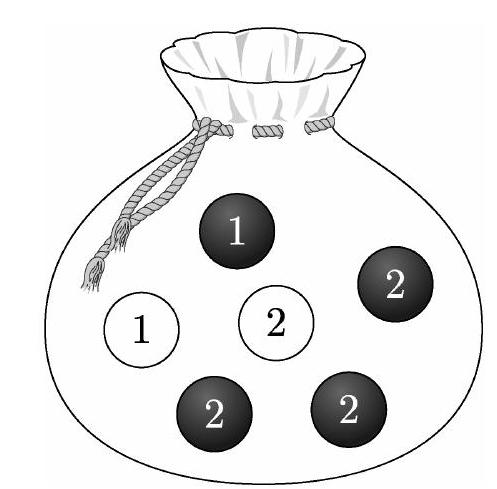
\includegraphics[max width=\textwidth]{2023_06_06_b380aa8523ec7afae994g-10}
\end{center}

\begin{enumerate}
  \setcounter{enumi}{26}
  \item 어느 회사에서 생산하는 샴푸 1 개의 용량은 정규분포 $\mathrm{N}\left(m, \sigma^{2}\right)$ 을 따른다고 한다. 이 회사에서 생산하는 샴푸 중에서 16 개를 임의추출하여 얻은 표본평균을 이용하여 구한 $m$ 에 대한 신뢰도 $95 \%$ 의 신뢰구간이 $746.1 \leq m \leq 755.9$ 이다.
\end{enumerate}

이 회사에서 생산하는 샴푸 중에서 $n$ 개를 임의추출하여 얻은 표본평균을 이용하여 구하는 $m$ 에 대한 신뢰도 $99 \%$ 의 신뢰구간이 $a \leq m \leq b$ 일 때, $b-a$ 의 값이 6 이하가 되기 위한 자연수 $n$ 의 최솟값은? (단, 용량의 단위는 $\mathrm{mL}$ 이고, $Z$ 가 표준정규분포를 따르는 확률변수일 때, $\mathrm{P}(|Z| \leq 1.96)=0.95$, $\mathrm{P}(|Z| \leq 2.58)=0.99$ 로 계산한다.) [3점]
(1) 70
(2) 74
(3) 78
(4) 82
(5) 86

\begin{enumerate}
  \setcounter{enumi}{27}
  \item 연속확률변수 $X$ 가 갖는 값의 범위는 $0 \leq X \leq a$ 이고, $X$ 의 확률밀도함수의 그래프가 그림과 같다.
\end{enumerate}

\begin{center}
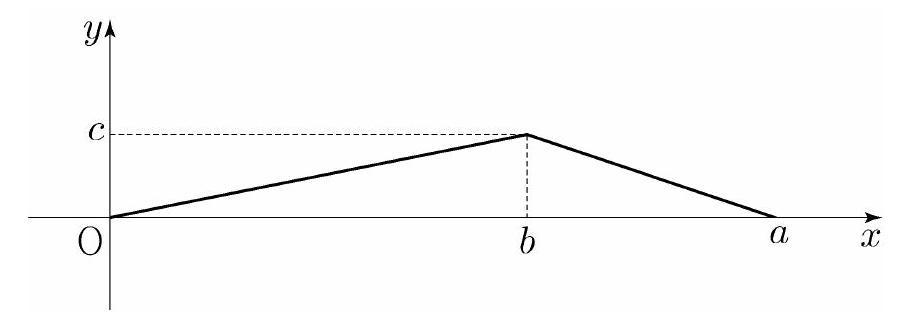
\includegraphics[max width=\textwidth]{2023_06_06_b380aa8523ec7afae994g-11}
\end{center}

$\mathrm{P}(X \leq b)-\mathrm{P}(X \geq b)=\frac{1}{4}, \mathrm{P}(X \leq \sqrt{5})=\frac{1}{2}$ 일 때, $a+b+c$ 의 값은? (단, $a, b, c$ 는 상수이다.) [4점]
(1) $\frac{11}{2}$
(2) 6
(3) $\frac{13}{2}$
(4) 7
(5) $\frac{15}{2}$

\section{4 수학 영역(확률과 통계)}
홀수형

\section{단답형}
\begin{enumerate}
  \setcounter{enumi}{28}
  \item 앞면에는 1 부터 6 까지의 자연수가 하나씩 적혀 있고 뒷면에는 모두 0 이 하나씩 적혀 있는 6 장의 카드가 있다. 이 6 장의 카드가 그림과 같이 6 이하의 자연수 $k$ 에 대하여 $k$ 번째 자리에 자연수 $k$ 가 보이도록 놓여 있다.
\end{enumerate}

\begin{center}
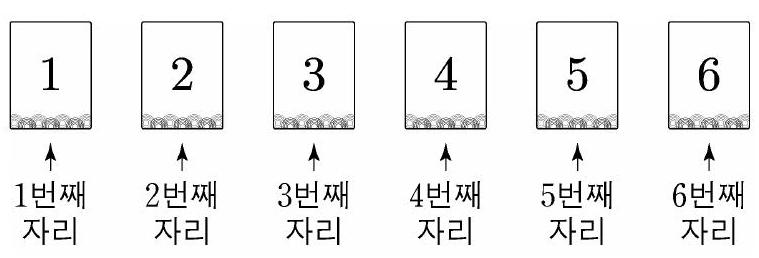
\includegraphics[max width=\textwidth]{2023_06_06_b380aa8523ec7afae994g-12}
\end{center}

이 6 장의 카드와 한 개의 주사위를 사용하여 다음 시행을 한다.

주사위를 한 번 던져 나온 눈의 수가 $k$ 이면

$k$ 번째 자리에 놓여 있는 카드를 한 번 뒤집어 제자리에 놓는다.

위의 시행을 3 번 반복한 후 6 장의 카드에 보이는 모든 수의 합이 짝수일 때, 주사위의 1 의 눈이 한 번만 나왔을 확률은 $\frac{q}{p}$ 이다. $p+q$ 의 값을 구하시오. (단, $p$ 와 $q$ 는 서로소인 자연수이다.) 30. 집합 $X=\{x \mid x$ 는 10 이하의 자연수 $\}$ 에 대하여 다음 조건을 만족시키는 함수 $f: X \rightarrow X$ 의 개수를 구하시오. [4점]

(가) 9 이하의 모든 자연수 $x$ 에 대하여 $f(x) \leq f(x+1)$ 이다.

(나) $1 \leq x \leq 5$ 일 때 $f(x) \leq x$ 이고, $6 \leq x \leq 10$ 일 때 $f(x) \geq x$ 이다.

(다) $f(6)=f(5)+6$ $*$ 확인 사항

○ 답안지의 해당란에 필요한 내용을 정확히 기입(표기)했는지 확인 하시오.

○ 이어서, 「선택과목(미적분)」 문제가 제시되오니, 자신이 선택한 과목인지 확인하시오. 제 2 교시

\section{3학년도 대학수학능력시험 문제지}
\section{수학 영역(미적분)}
홀수형

5지선다형

\begin{enumerate}
  \setcounter{enumi}{22}
  \item $\lim _{x \rightarrow 0} \frac{\ln (x+1)}{\sqrt{x+4}-2}$ 의 값은? [2점]
(1) 1
(2) 2
(3) 3
(4) 4
(5) 5

  \item $\lim _{n \rightarrow \infty} \frac{1}{n} \sum_{k=1}^{n} \sqrt{1+\frac{3 k}{n}}$ 의 값은? [3점]
(1) $\frac{4}{3}$
(2) $\frac{13}{9}$
(3) $\frac{14}{9}$
(4) $\frac{5}{3}$
(5) $\frac{16}{9}$ 25. 등비수열 $\left\{a_{n}\right\}$ 에 대하여 $\lim _{n \rightarrow \infty} \frac{a_{n}+1}{3^{n}+2^{2 n-1}}=3$ 일 때, $a_{2}$ 의 값은? [3점]
(1) 16
(2) 18
(3) 20
(4) 22
(5) 24

  \item 그림과 같이 곡선 $y=\sqrt{\sec ^{2} x+\tan x}\left(0 \leq x \leq \frac{\pi}{3}\right)$ 와 $x$ 축, $y$ 축 및 직선 $x=\frac{\pi}{3}$ 로 둘러싸인 부분을 밑면으로 하는 입체도형이 있다. 이 입체도형을 $x$ 축에 수직인 평면으로 자른 단면이 모두 정사각형일 때, 이 입체도형의 부피는? [3점]

\end{enumerate}

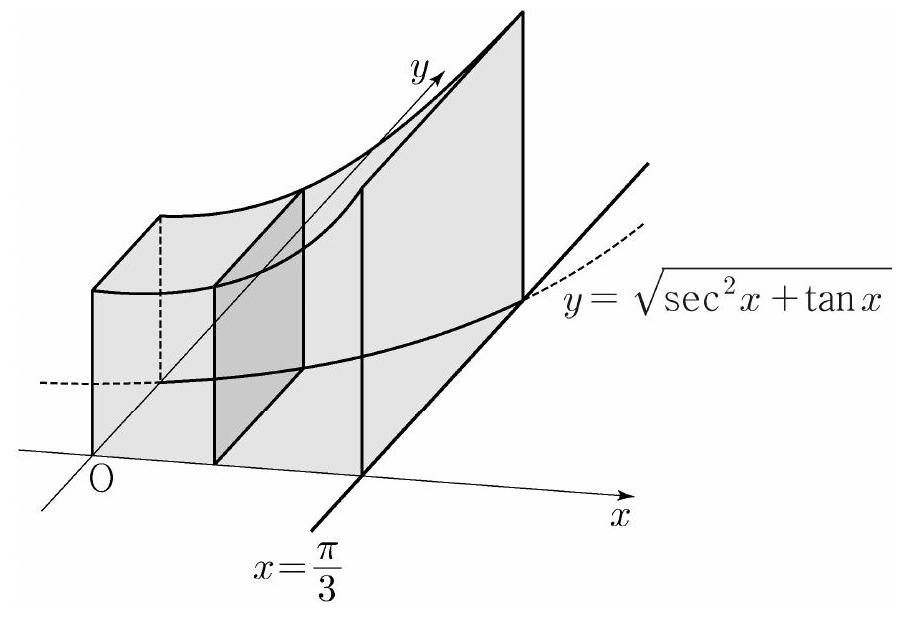
\includegraphics[max width=\textwidth, center]{2023_06_06_b380aa8523ec7afae994g-14}
(1) $\frac{\sqrt{3}}{2}+\frac{\ln 2}{2}$
(2) $\frac{\sqrt{3}}{2}+\ln 2$
(3) $\sqrt{3}+\frac{\ln 2}{2}$
(4) $\sqrt{3}+\ln 2$
(5) $\sqrt{3}+2 \ln 2$ 27. 그림과 같이 중심이 $\mathrm{O}$, 반지름의 길이가 1 이고 중심각의 크기가 $\frac{\pi}{2}$ 인 부채꼴 $\mathrm{OA}_{1} \mathrm{~B}_{1}$ 이 있다. 호 $\mathrm{A}_{1} \mathrm{~B}_{1}$ 위에 점 $\mathrm{P}_{1}$, 선분 $\mathrm{OA}_{1}$ 위에 점 $\mathrm{C}_{1}$, 선분 $\mathrm{OB}_{1}$ 위에 점 $\mathrm{D}_{1}$ 을 사각형 $\mathrm{OC}_{1} \mathrm{P}_{1} \mathrm{D}_{1}$ 이 $\overline{\mathrm{OC}_{1}}: \overline{\mathrm{OD}_{1}}=3: 4$ 인 직사각형이 되도록 잡는다. 부채꼴 $\mathrm{OA}_{1} \mathrm{~B}_{1}$ 의 내부에 점 $\mathrm{Q}_{1}$ 을 $\overline{\mathrm{P}_{1} \mathrm{Q}_{1}}=\overline{\mathrm{A}_{1} \mathrm{Q}_{1}}, \angle \mathrm{P}_{1} \mathrm{Q}_{1} \mathrm{~A}_{1}=\frac{\pi}{2}$ 가 되도록 잡고, 이등변삼각형 $\mathrm{P}_{1} \mathrm{Q}_{1} \mathrm{~A}_{1}$ 에 색칠하여 얻은 그림을 $R_{1}$ 이라 하자.

그림 $R_{1}$ 에서 선분 $\mathrm{OA}_{1}$ 위의 점 $\mathrm{A}_{2}$ 와 선분 $\mathrm{OB}_{1}$ 위의 점 $\mathrm{B}_{2}$ 를 $\overline{\mathrm{OQ}_{1}}=\overline{\mathrm{OA}_{2}}=\overline{\mathrm{OB}_{2}}$ 가 되도록 잡고, 중심이 $\mathrm{O}$, 반지름의 길이가 $\overline{\mathrm{OQ}_{1}}$, 중심각의 크기가 $\frac{\pi}{2}$ 인 부채꼴 $\mathrm{OA}_{2} \mathrm{~B}_{2}$ 를 그린다. 그림 $R_{1}$ 을 얻은 것과 같은 방법으로 네 점 $\mathrm{P}_{2}, \mathrm{C}_{2}, \mathrm{D}_{2}, \mathrm{Q}_{2}$ 를 잡고, 이등변삼각형 $\mathrm{P}_{2} \mathrm{Q}_{2} \mathrm{~A}_{2}$ 에 색칠하여 얻은 그림을 $R_{2}$ 라 하자. 이와 같은 과정을 계속하여 $n$ 번째 얻은 그림 $R_{n}$ 에 색칠되어 있는 부분의 넓이를 $S_{n}$ 이라 할 때, $\lim _{n \rightarrow \infty} S_{n}$ 의 값은? [3점]
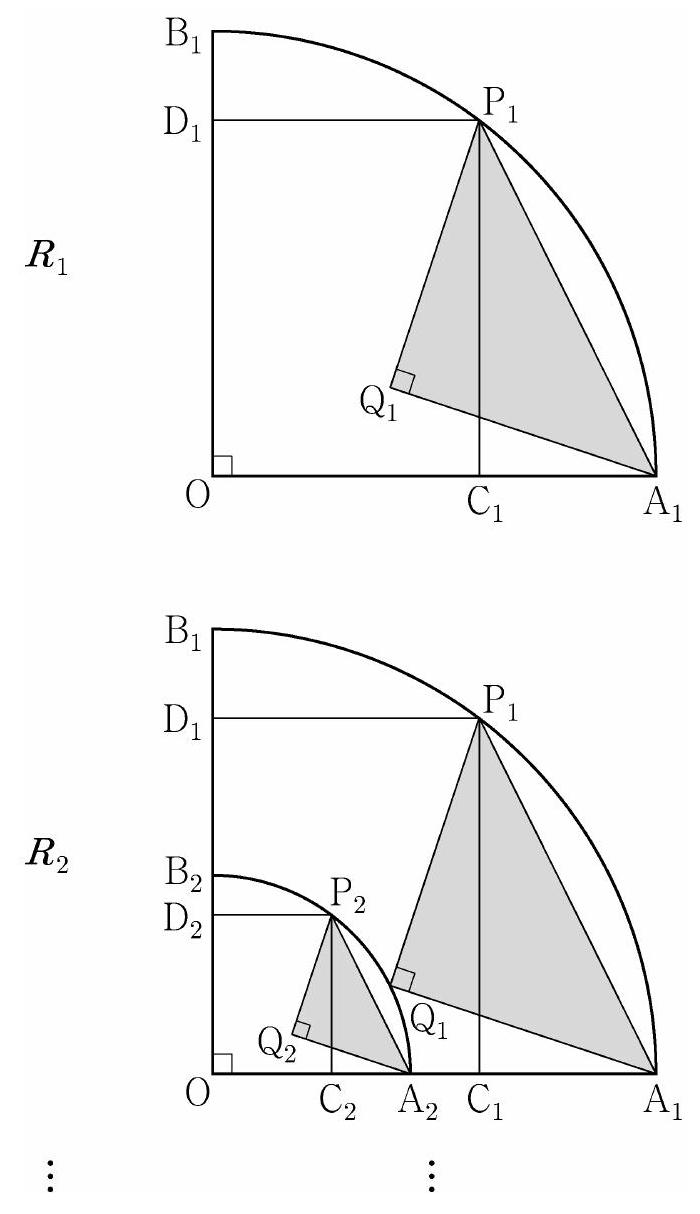
\includegraphics[max width=\textwidth, center]{2023_06_06_b380aa8523ec7afae994g-15(1)}
(1) $\frac{9}{40}$
(2) $\frac{1}{4}$
(3) $\frac{11}{40}$
(4) $\frac{3}{10}$
(5) $\frac{13}{40}$

\begin{enumerate}
  \setcounter{enumi}{27}
  \item 그림과 같이 중심이 $\mathrm{O}$ 이고 길이가 2 인 선분 $\mathrm{AB}$ 를 지름으로 하는 반원 위에 $\angle \mathrm{AOC}=\frac{\pi}{2}$ 인 점 $\mathrm{C}$ 가 있다. 호 $\mathrm{BC}$ 위에 점 $\mathrm{P}$ 와 호 $\mathrm{CA}$ 위에 점 $\mathrm{Q}$ 를 $\overline{\mathrm{PB}}=\overline{\mathrm{QC}}$ 가 되도록 잡고, 선분 $\mathrm{AP}$ 위에 점 $\mathrm{R}$ 를 $\angle \mathrm{CQR}=\frac{\pi}{2}$ 가 되도록 잡는다. 선분 $\mathrm{AP}$ 와 선분 $\mathrm{CO}$ 의 교점을 $\mathrm{S}$ 라 하자. $\angle \mathrm{PAB}=\theta$ 일 때, 삼각형 $\mathrm{POB}$ 의 넓이를 $f(\theta)$, 사각형 $\mathrm{CQRS}$ 의 넓이를 $g(\theta)$ 라 하자. $\lim _{\theta \rightarrow 0+} \frac{3 f(\theta)-2 g(\theta)}{\theta^{2}}$ 의 값은? (단, $0<\theta<\frac{\pi}{4}$ ) [4점]
\end{enumerate}

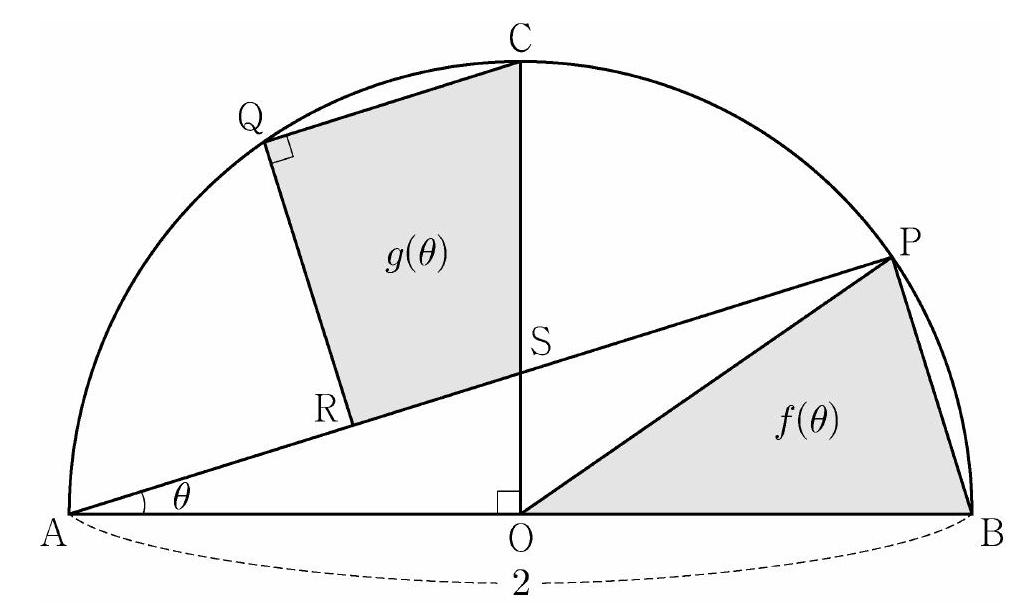
\includegraphics[max width=\textwidth, center]{2023_06_06_b380aa8523ec7afae994g-15}
(1) 1
(2) 2
(3) 3
(4) 4
(5) 5

\section{단답형}
\begin{enumerate}
  \setcounter{enumi}{28}
  \item 세 상수 $a, b, c$ 에 대하여 함수 $f(x)=a e^{2 x}+b e^{x}+c$ 가 다음 조건을 만족시킨다.
\end{enumerate}

$$
\begin{aligned}
& \text { (가) } \lim _{x \rightarrow-\infty} \frac{f(x)+6}{e^{x}}=1 \\
& \text { (나) } f(\ln 2)=0
\end{aligned}
$$

함수 $f(x)$ 의 역함수를 $g(x)$ 라 할 때, $\int_{0}^{14} g(x) d x=p+q \ln 2$ 이다. $p+q$ 의 값을 구하시오. (단, $p, q$ 는 유리수이고, $\ln 2$ 는 무리수이다.) [4점] 30. 최고차항의 계수가 양수인 삼차함수 $f(x)$ 와 함수 $g(x)=e^{\sin \pi x}-1$ 에 대하여 실수 전체의 집합에서 정의된 합성함수 $h(x)=g(f(x))$ 가 다음 조건을 만족시킨다.

(가) 함수 $h(x)$ 는 $x=0$ 에서 극댓값 0 을 갖는다.

(나) 열린구간 $(0,3)$ 에서 방정식 $h(x)=1$ 의 서로 다른 실근의 개수는 7 이다.

$f(3)=\frac{1}{2}, f^{\prime}(3)=0$ 일 때, $f(2)=\frac{q}{p}$ 이다. $p+q$ 의 값을 구하시오. (단, $p$ 와 $q$ 는 서로소인 자연수이다.) [4점] * 확인 사항

○ 답안지의 해당란에 필요한 내용을 정확히 기입(표기)했는지 확인 하시오.

○ 이어서, 「선택과목(기하)」 문제가 제시되오니, 자신이 선택한 과목인지 확인하시오. 제 2 교시

\section{3학년도 대학수학능력시험 문제지}
\section{수학 영역(기하)}
홀수형

\section{5 지선다형}
\begin{enumerate}
  \setcounter{enumi}{22}
  \item 좌표공간의 점 $\mathrm{A}(2,2,-1)$ 을 $x$ 축에 대하여 대칭이동한 점을 $\mathrm{B}$ 라 하자. 점 $\mathrm{C}(-2,1,1)$ 에 대하여 선분 $\mathrm{BC}$ 의 길이는?
\end{enumerate}

[2점]
(1) 1
(2) 2
(3) 3
(4) 4
(5) 5

\begin{enumerate}
  \setcounter{enumi}{23}
  \item 초점이 $\mathrm{F}\left(\frac{1}{3}, 0\right)$ 이고 준선이 $x=-\frac{1}{3}$ 인 포물선이 점 $(a, 2)$ 를 지날 때, $a$ 의 값은? [3점]
(1) 1
(2) 2
(3) 3
(4) 4
(5) 5 25. 타원 $\frac{x^{2}}{a^{2}}+\frac{y^{2}}{b^{2}}=1$ 위의 점 $(2,1)$ 에서의 접선의 기울기가 $-\frac{1}{2}$ 일 때, 이 타원의 두 초점 사이의 거리는? (단, $a, b$ 는 양수이다.) [3점]
(1) $2 \sqrt{3}$
(2) 4
(3) $2 \sqrt{5}$
(4) $2 \sqrt{6}$
(5) $2 \sqrt{7}$

  \item 좌표평면에서 세 벡터

\end{enumerate}

$$
\vec{a}=(2,4), \quad \vec{b}=(2,8), \quad \vec{c}=(1,0)
$$

에 대하여 두 벡터 $\vec{p}, \vec{q}$ 가

$$
(\vec{p}-\vec{a}) \cdot(\vec{p}-\vec{b})=0, \quad \vec{q}=\frac{1}{2} \vec{a}+t \vec{c}(t \text { 는 실수 })
$$

를 만족시킬 때, $|\vec{p}-\vec{q}|$ 의 최솟값은? [3점]
(1) $\frac{3}{2}$
(2) 2
(3) $\frac{5}{2}$
(4) 3
(5) $\frac{7}{2}$ 27. 좌표공간에 직선 $\mathrm{AB}$ 를 포함하는 평면 $\alpha$ 가 있다. 평면 $\alpha$ 위에 있지 않은 점 $\mathrm{C}$ 에 대하여 직선 $\mathrm{AB}$ 와 직선 $\mathrm{AC}$ 가 이루는 예각의 크기를 $\theta_{1}$ 이라 할 때 $\sin \theta_{1}=\frac{4}{5}$ 이고, 직선 $\mathrm{AC}$ 와 평면 $\alpha$ 가 이루는 예각의 크기는 $\frac{\pi}{2}-\theta_{1}$ 이다. 평면 $\mathrm{ABC}$ 와 평면 $\alpha$ 가 이루는 예각의 크기를 $\theta_{2}$ 라 할 때, $\cos \theta_{2}$ 의 값은? [3점]
(1) $\frac{\sqrt{7}}{4}$
(2) $\frac{\sqrt{7}}{5}$
(3) $\frac{\sqrt{7}}{6}$
(4) $\frac{\sqrt{7}}{7}$
(5) $\frac{\sqrt{7}}{8}$

\begin{center}
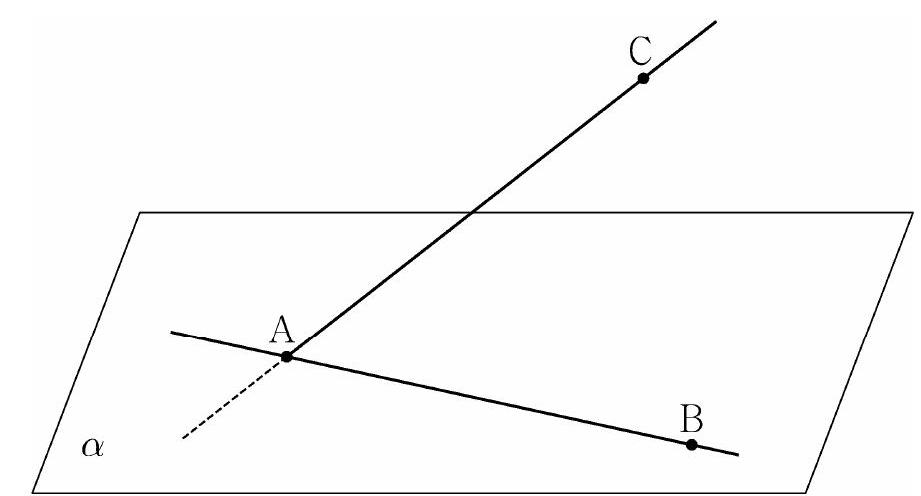
\includegraphics[max width=\textwidth]{2023_06_06_b380aa8523ec7afae994g-19(1)}
\end{center}

\begin{enumerate}
  \setcounter{enumi}{27}
  \item 두 초점이 $\mathrm{F}(c, 0), \mathrm{F}^{\prime}(-c, 0)(c>0)$ 인 쌍곡선 $C$ 와 $y$ 축 위의 점 $\mathrm{A}$ 가 있다. 쌍곡선 $C$ 가 선분 $\mathrm{AF}$ 와 만나는 점을 $\mathrm{P}$, 선분 $\mathrm{AF}^{\prime}$ 과 만나는 점을 $\mathrm{P}^{\prime}$ 이라 하자.
\end{enumerate}

직선 $\mathrm{AF}$ 는 쌍곡선 $C$ 의 한 점근선과 평행하고

$$
\overline{\mathrm{AP}}: \overline{\mathrm{PP}^{\prime}}=5: 6, \quad \overline{\mathrm{PF}}=1
$$

일 때, 쌍곡선 $C$ 의 주축의 길이는? [4점]
(1) $\frac{13}{6}$
(2) $\frac{9}{4}$
(3) $\frac{7}{3}$
(4) $\frac{29}{12}$
(5) $\frac{5}{2}$

\begin{center}
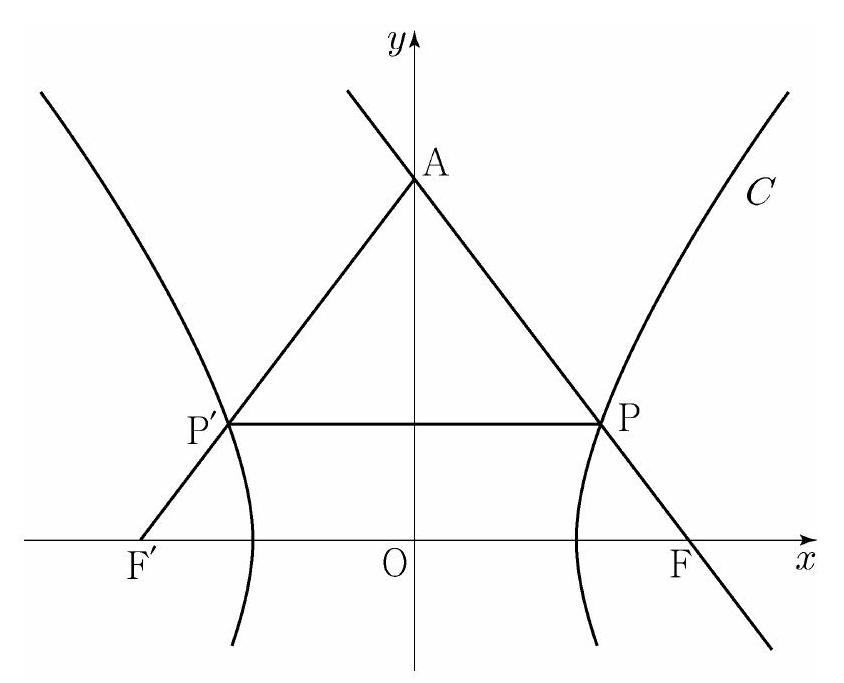
\includegraphics[max width=\textwidth]{2023_06_06_b380aa8523ec7afae994g-19}
\end{center}

\section{4 수학 영역(기하)}
홀수형

\section{단답 형}
\begin{enumerate}
  \setcounter{enumi}{28}
  \item 평면 $\alpha$ 위에 $\overline{\mathrm{AB}}=\overline{\mathrm{CD}}=\overline{\mathrm{AD}}=2, \angle \mathrm{ABC}=\angle \mathrm{BCD}=\frac{\pi}{3}$ 인 사다리꼴 $\mathrm{ABCD}$ 가 있다. 다음 조건을 만족시키는 평면 $\alpha$ 위의 두 점 $\mathrm{P}, \mathrm{Q}$ 에 대하여 $\overrightarrow{\mathrm{CP}} \cdot \overrightarrow{\mathrm{DQ}}$ 의 값을 구하시오. [4점]
(가) $\overrightarrow{\mathrm{AC}}=2(\overrightarrow{\mathrm{AD}}+\overrightarrow{\mathrm{BP}})$
(나) $\overrightarrow{\mathrm{AC}} \cdot \overrightarrow{\mathrm{PQ}}=6$
(다) $2 \times \angle \mathrm{BQA}=\angle \mathrm{PBQ}<\frac{\pi}{2}$
\end{enumerate}

\begin{center}
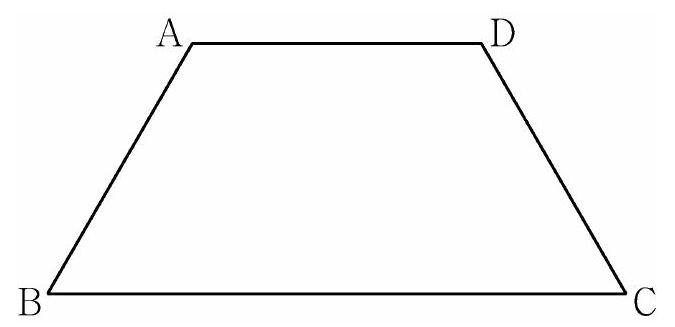
\includegraphics[max width=\textwidth]{2023_06_06_b380aa8523ec7afae994g-20}
\end{center}

\begin{enumerate}
  \setcounter{enumi}{29}
  \item 좌표공간에 정사면체 $\mathrm{ABCD}$ 가 있다. 정삼각형 $\mathrm{BCD}$ 의 외심을 중심으로 하고 점 $\mathrm{B}$ 를 지나는 구를 $S$ 라 하자. 구 $S$ 와 선분 $\mathrm{AB}$ 가 만나는 점 중 $\mathrm{B}$ 가 아닌 점을 $\mathrm{P}$, 구 $S$ 와 선분 $\mathrm{AC}$ 가 만나는 점 중 $\mathrm{C}$ 가 아닌 점을 $\mathrm{Q}$, 구 $S$ 와 선분 $\mathrm{AD}$ 가 만나는 점 중 $\mathrm{D}$ 가 아닌 점을 $\mathrm{R}$ 라 하고, 점 $\mathrm{P}$ 에서 구 $S$ 에 접하는 평면을 $\alpha$ 라 하자. 구 $S$ 의 반지름의 길이가 6 일 때, 삼각형 $\mathrm{PQR}$ 의 평면 $\alpha$ 위로의 정사영의 넓이는 $k$ 이다. $k^{2}$ 의 값을 구하시오. [4점]
\end{enumerate}

\begin{center}
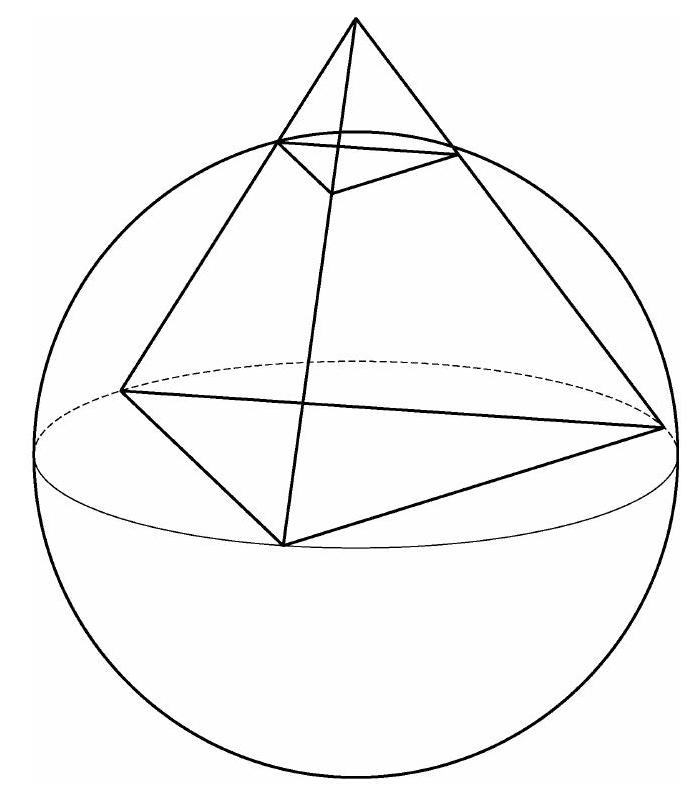
\includegraphics[max width=\textwidth]{2023_06_06_b380aa8523ec7afae994g-20(1)}
\end{center}

\begin{itemize}
  \item 확인 사항
\end{itemize}

○ 답안지의 해당란에 필요한 내용을 정확히 기입(표기)했는지 확인 하시오.

\section{3학년도 대학수학능력시험 문제지}
제 2 교시

\section{수하 영여}
짝수형

\section{5 지선다형}
\begin{enumerate}
  \item $\left(\frac{4}{2^{\sqrt{2}}}\right)^{2+\sqrt{2}}$ 의 값은? [2점]
(1) $\frac{1}{4}$
(2) $\frac{1}{2}$
(3) 1
(4) 2
(5) 4

  \item $\lim _{x \rightarrow \infty} \frac{\sqrt{x^{2}-2}+3 x}{x+5}$ 의 값은? [2점]
(1) 1
(2) 2
(3) 3
(4) 4
(5) 5

  \item 공비가 양수인 등비수열 $\left\{a_{n}\right\}$ 이

\end{enumerate}

$$
a_{2}+a_{4}=30, \quad a_{4}+a_{6}=\frac{15}{2}
$$

를 만족시킬 때, $a_{1}$ 의 값은? [3점]
(1) 48
(2) 56
(3) 64
(4) 72
(5) 80

\begin{enumerate}
  \setcounter{enumi}{3}
  \item 다항함수 $f(x)$ 에 대하여 함수 $g(x)$ 를
\end{enumerate}

$$
g(x)=x^{2} f(x)
$$

라 하자. $f(2)=1, f^{\prime}(2)=3$ 일 때, $g^{\prime}(2)$ 의 값은? [3점]
(1) 12
(2) 14
(3) 16
(4) 18
(5) 20 5. $\tan \theta<0$ 이고 $\cos \left(\frac{\pi}{2}+\theta\right)=\frac{\sqrt{5}}{5}$ 일 때, $\cos \theta$ 의 값은? [3점]
(1) $-\frac{2 \sqrt{5}}{5}$
(2) $-\frac{\sqrt{5}}{5}$
(3) 0
(4) $\frac{\sqrt{5}}{5}$
(5) $\frac{2 \sqrt{5}}{5}$

\begin{enumerate}
  \setcounter{enumi}{5}
  \item 함수 $f(x)=2 x^{3}-9 x^{2}+a x+5$ 는 $x=1$ 에서 극대이고, $x=b$ 에서 극소이다. $a+b$ 의 값은? (단, $a, b$ 는 상수이다.) [3점]
(1) 12
(2) 14
(3) 16
(4) 18
(5) 20

  \item 모든 항이 양수이고 첫째항과 공차가 같은 등차수열 $\left\{a_{n}\right\}$ 이

\end{enumerate}

$$
\sum_{k=1}^{15} \frac{1}{\sqrt{a_{k}}+\sqrt{a_{k+1}}}=2
$$

를 만족시킬 때, $a_{4}$ 의 값은? [3점]
(1) 6
(2) 7
(3) 8
(4) 9
(5) 10 8. 점 $(0,4)$ 에서 곡선 $y=x^{3}-x+2$ 에 그은 접선의 $x$ 절편은?

[3점]
(1) $-\frac{5}{2}$
(2) -2
(3) $-\frac{3}{2}$
(4) -1
(5) $-\frac{1}{2}$

\begin{enumerate}
  \setcounter{enumi}{8}
  \item 함수
\end{enumerate}

$$
f(x)=a-\sqrt{3} \tan 2 x
$$

가 닫힌구간 $\left[-\frac{\pi}{6}, b\right]$ 에서 최댓값 7 , 최솟값 3 을 가질 때, $a \times b$ 의 값은? (단, $a, b$ 는 상수이다.) [4점]
(1) $\frac{\pi}{2}$
(2) $\frac{5 \pi}{12}$
(3) $\frac{\pi}{3}$
(4) $\frac{\pi}{4}$
(5) $\frac{\pi}{6}$

\begin{enumerate}
  \setcounter{enumi}{9}
  \item 두 곡선 $y=x^{3}+x^{2}, y=-x^{2}+k$ 와 $y$ 축으로 둘러싸인 부분의 넓이를 $A$, 두 곡선 $y=x^{3}+x^{2}, y=-x^{2}+k$ 와 직선 $x=2$ 로 둘러싸인 부분의 넓이를 $B$ 라 하자. $A=B$ 일 때, 상수 $k$ 의 값은? (단, $4<k<5$ ) [4점]
(1) $\frac{25}{6}$
(2) $\frac{13}{3}$
(3) $\frac{9}{2}$
(4) $\frac{14}{3}$
(5) $\frac{29}{6}$
\end{enumerate}

\begin{center}
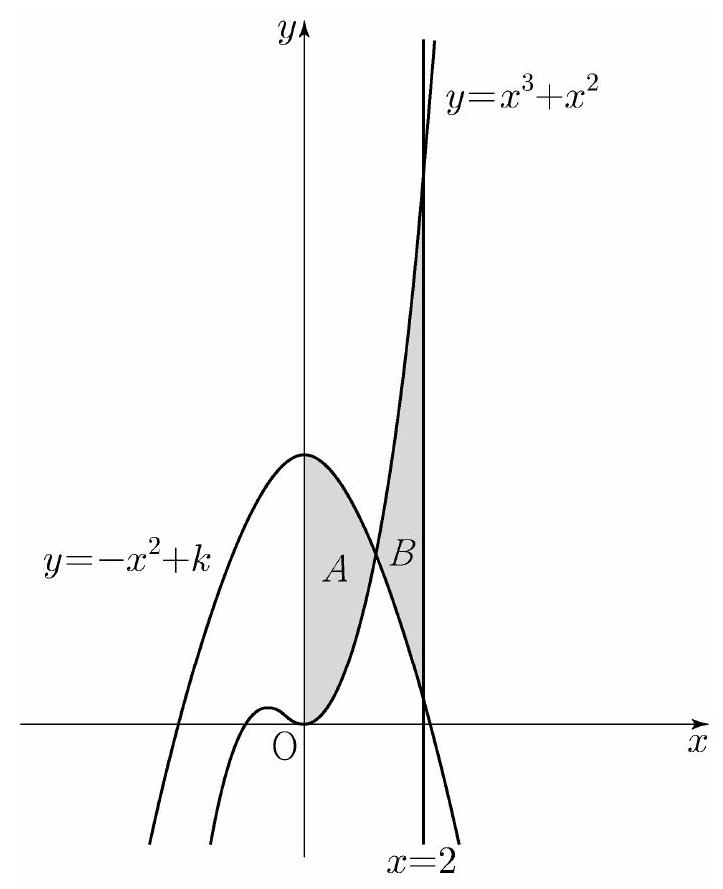
\includegraphics[max width=\textwidth]{2023_06_06_b380aa8523ec7afae994g-23}
\end{center}

\begin{enumerate}
  \setcounter{enumi}{10}
  \item 그림과 같이 사각형 $\mathrm{ABCD}$ 가 한 원에 내접하고
\end{enumerate}

$$
\overline{\mathrm{AB}}=5, \overline{\mathrm{AC}}=3 \sqrt{5}, \overline{\mathrm{AD}}=7, \angle \mathrm{BAC}=\angle \mathrm{CAD}
$$

일 때, 이 원의 반지름의 길이는? [4점]

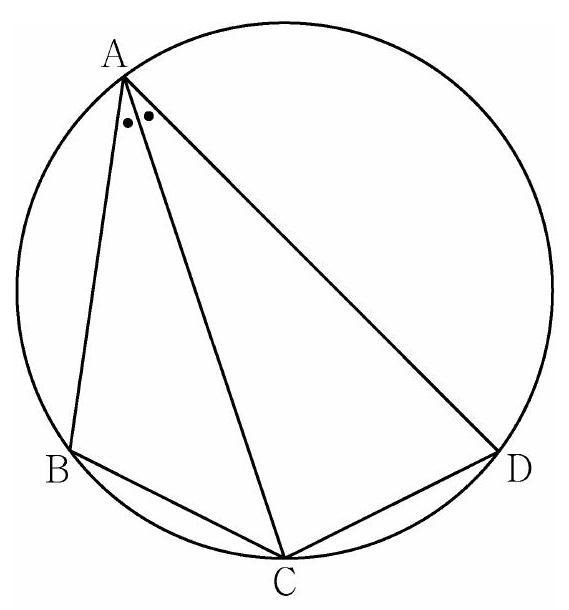
\includegraphics[max width=\textwidth, center]{2023_06_06_b380aa8523ec7afae994g-24}
(1) $\frac{5 \sqrt{2}}{2}$
(2) $\frac{8 \sqrt{5}}{5}$
(3) $\frac{5 \sqrt{5}}{3}$
(4) $\frac{8 \sqrt{2}}{3}$
(5) $\frac{9 \sqrt{3}}{4}$

\begin{enumerate}
  \setcounter{enumi}{11}
  \item 실수 전체의 집합에서 연속인 함수 $f(x)$ 가 다음 조건을 만족시킨다.
\end{enumerate}

$n-1 \leq x<n$ 일 때, $|f(x)|=|6(x-n+1)(x-n)|$ 이다. (단, $n$ 은 자연수이다.)

열린구간 $(0,4)$ 에서 정의된 함수

$$
g(x)=\int_{0}^{x} f(t) d t-\int_{x}^{4} f(t) d t
$$

가 $x=2$ 에서 최솟값 0 을 가질 때, $\int_{\frac{1}{2}}^{4} f(x) d x$ 의 값은? [4점]
(1) $\frac{5}{2}$
(2) $\frac{3}{2}$
(3) $\frac{1}{2}$
(4) $-\frac{1}{2}$
(5) $-\frac{3}{2}$ 13. 자연수 $m(m \geq 2)$ 에 대하여 $m^{12}$ 의 $n$ 제곱근 중에서 정수가 존재하도록 하는 2 이상의 자연수 $n$ 의 개수를 $f(m)$ 이라 할 때, $\sum_{m=2}^{9} f(m)$ 의 값은? [4점]
(1) 37
(2) 42
(3) 47
(4) 52
(5) 57

\begin{enumerate}
  \setcounter{enumi}{13}
  \item 다항함수 $f(x)$ 에 대하여 함수 $g(x)$ 를 다음과 같이 정의한다.
\end{enumerate}

$$
g(x)= \begin{cases}x & (x<-1 \text { 또는 } x>1) \\ f(x) & (-1 \leq x \leq 1)\end{cases}
$$

함수 $h(x)=\lim _{t \rightarrow 0+} g(x+t) \times \lim _{t \rightarrow 2+} g(x+t)$ 에 대하여

<보기>에서 옳은 것만을 있는 대로 고른 것은? [4점]

ᄀ. $h(1)=3$

ㄴ. 함수 $h(x)$ 는 실수 전체의 집합에서 연속이다.

ㄷ. 함수 $g(x)$ 가 닫힌구간 $[-1,1]$ 에서 감소하고 $g(-1)=-2$ 이면 함수 $h(x)$ 는 실수 전체의 집합에서 최솟값을 갖는다.
(1) ᄀ
(2) 1
(3) ᄀ, ᄂ (4) ᄀ, ᄃ
(5) ᄂ, ᄃ 15. 모든 항이 자연수이고 다음 조건을 만족시키는 모든 수열 $\left\{a_{n}\right\}$ 에 대하여 $a_{9}$ 의 최댓값과 최솟값을 각각 $M, m$ 이라 할 때, $M+m$ 의 값은? [4점]

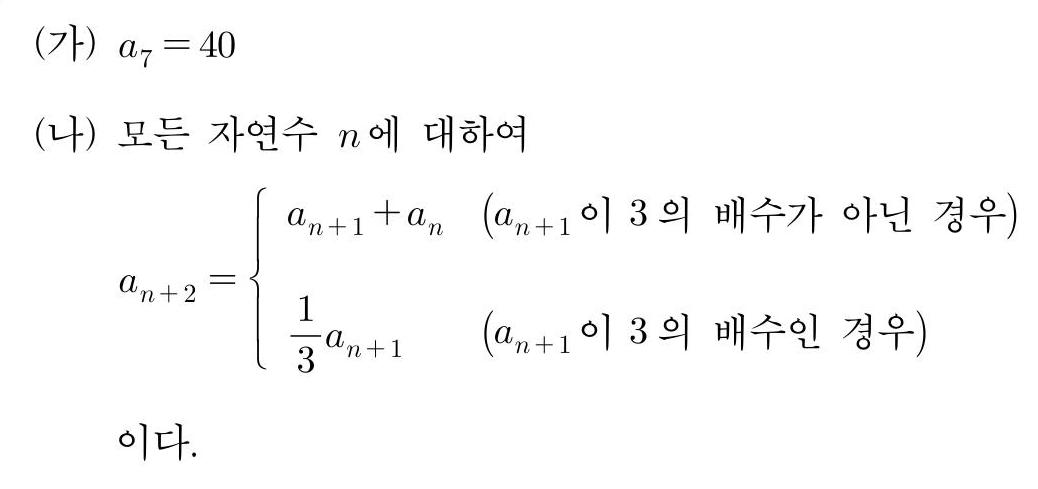
\includegraphics[max width=\textwidth, center]{2023_06_06_b380aa8523ec7afae994g-26}
(1) 216
(2) 218
(3) 220
(4) 222
(5) 224

\section{단 답형}
\begin{enumerate}
  \setcounter{enumi}{15}
  \item 방정식
\end{enumerate}

$$
\log _{2}(3 x+2)=2+\log _{2}(x-2)
$$

를 만족시키는 실수 $x$ 의 값을 구하시오. [3점]

\begin{enumerate}
  \setcounter{enumi}{16}
  \item 함수 $f(x)$ 에 대하여 $f^{\prime}(x)=4 x^{3}-2 x$ 이고 $f(0)=3$ 일 때, $f(2)$ 의 값을 구하시오. [3점] 18. 두 수열 $\left\{a_{n}\right\},\left\{b_{n}\right\}$ 에 대하여
\end{enumerate}

$$
\sum_{k=1}^{5}\left(3 a_{k}+5\right)=55, \quad \sum_{k=1}^{5}\left(a_{k}+b_{k}\right)=32
$$

일 때, $\sum_{k=1}^{5} b_{k}$ 의 값을 구하시오. [3점]

\begin{enumerate}
  \setcounter{enumi}{18}
  \item 방정식 $2 x^{3}-6 x^{2}+k=0$ 의 서로 다른 양의 실근의 개수가 2 가 되도록 하는 정수 $k$ 의 개수를 구하시오. [3점] 20. 수직선 위를 움직이는 점 $\mathrm{P}$ 의 시각 $t(t \geq 0)$ 에서의 속도 $v(t)$ 와 가속도 $a(t)$ 가 다음 조건을 만족시킨다.
\end{enumerate}

(가) $0 \leq t \leq 2$ 일 때, $v(t)=2 t^{3}-8 t$ 이다.

(나) $t \geq 2$ 일 때, $a(t)=6 t+4$ 이다.

시각 $t=0$ 에서 $t=3$ 까지 점 $\mathrm{P}$ 가 움직인 거리를 구하시오. [4점] 21. 자연수 $n$ 에 대하여 함수 $f(x)$ 를

$$
f(x)= \begin{cases}\left|3^{x+2}-n\right| & (x<0) \\ \left|\log _{2}(x+4)-n\right| & (x \geq 0)\end{cases}
$$

이라 하자. 실수 $t$ 에 대하여 $x$ 에 대한 방정식 $f(x)=t$ 의 서로 다른 실근의 개수를 $g(t)$ 라 할 때, 함수 $g(t)$ 의 최댓값이 4 가 되도록 하는 모든 자연수 $n$ 의 값의 합을 구하시오. [4점] 22. 최고차항의 계수가 1 인 삼차함수 $f(x)$ 와 실수 전체의 집합에서 연속인 함수 $g(x)$ 가 다음 조건을 만족시킬 때, $f(4)$ 의 값을 구하시오. [4점]

(가) 모든 실수 $x$ 에 대하여

$$
f(x)=f(1)+(x-1) f^{\prime}(g(x)) \text { 이다. }
$$

(나) 함수 $g(x)$ 의 최솟값은 $\frac{5}{2}$ 이다.

(다) $f(0)=-3, f(g(1))=6$

\section{* 확인 사항}
○ 답안지의 해당란에 필요한 내용을 정확히 기입(표기)했는지 확인 하시오.

○ 이어서, 「선택과목(확률과 통계)」 문제가 제시되오니, 자신이 선택한 과목인지 확인하시오.

\section{3학년도 대학수학능력시험 문제지
제2교시 수학 영역(확률과 통계)
짝수형}
\section{5 지선다형}
\begin{enumerate}
  \setcounter{enumi}{22}
  \item 다항식 $\left(x^{3}+3\right)^{5}$ 의 전개식에서 $x^{9}$ 의 계수는? [2점]
(1) 30
(2) 60
(3) 90
(4) 120
(5) 150

  \item 숫자 $1,2,3,4,5$ 중에서 중복을 허락하여 4 개를 택해 일렬로 나열하여 만들 수 있는 네 자리의 자연수 중 4000 이상인 홀수의 개수는? [3점]
(1) 125
(2) 150
(3) 175
(4) 200
(5) 225 25. 흰색 마스크 5 개, 검은색 마스크 9 개가 들어 있는 상자가 있다. 이 상자에서 임의로 3 개의 마스크를 동시에 꺼낼 때, 꺼낸 3 개의 마스크 중에서 적어도 한 개가 흰색 마스크일 확률은? [3점]
(1) $\frac{8}{13}$
(2) $\frac{17}{26}$
(3) $\frac{9}{13}$
(4) $\frac{19}{26}$
(5) $\frac{10}{13}$

  \item 주머니에 1 이 적힌 흰 공 1 개, 2 가 적힌 흰 공 1 개, 1 이 적힌 검은 공 1 개, 2 가 적힌 검은 공 3 개가 들어 있다. 이 주머니에서 임의로 3 개의 공을 동시에 꺼내는 시행을 한다. 이 시행에서 꺼낸 3 개의 공 중에서 흰 공이 1 개이고 검은 공이 2 개인 사건을 $A$, 꺼낸 3 개의 공에 적혀 있는 수를 모두 곱한 값이 8 인 사건을 $B$ 라 할 때, $\mathrm{P}(A \cup B)$ 의 값은? [3점]
(1) $\frac{11}{20}$
(2) $\frac{3}{5}$
(3) $\frac{13}{20}$
(4) $\frac{7}{10}$
(5) $\frac{3}{4}$

\end{enumerate}

\begin{center}
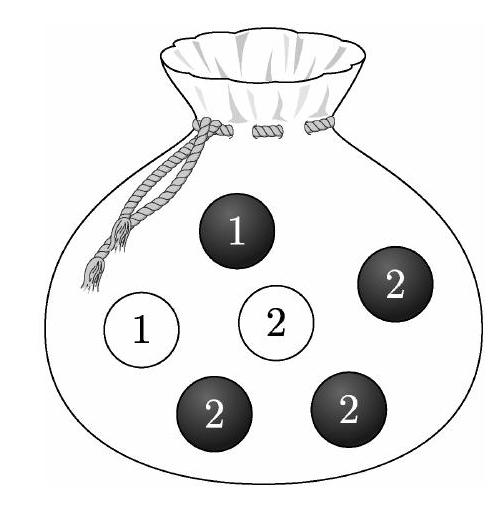
\includegraphics[max width=\textwidth]{2023_06_06_b380aa8523ec7afae994g-30}
\end{center}

\begin{enumerate}
  \setcounter{enumi}{26}
  \item 어느 회사에서 생산하는 샴푸 1 개의 용량은 정규분포 $\mathrm{N}\left(m, \sigma^{2}\right)$ 을 따른다고 한다. 이 회사에서 생산하는 샴푸 중에서 16 개를 임의추출하여 얻은 표본평균을 이용하여 구한 $m$ 에 대한 신뢰도 $95 \%$ 의 신뢰구간이 $746.1 \leq m \leq 755.9$ 이다.
\end{enumerate}

이 회사에서 생산하는 샴푸 중에서 $n$ 개를 임의추출하여 얻은 표본평균을 이용하여 구하는 $m$ 에 대한 신뢰도 $99 \%$ 의 신뢰구간이 $a \leq m \leq b$ 일 때, $b-a$ 의 값이 6 이하가 되기 위한 자연수 $n$ 의 최솟값은? (단, 용량의 단위는 $\mathrm{mL}$ 이고, $Z$ 가 표준정규분포를 따르는 확률변수일 때, $\mathrm{P}(|Z| \leq 1.96)=0.95$, $\mathrm{P}(|Z| \leq 2.58)=0.99$ 로 계산한다.) [3점]
(1) 70
(2) 74
(3) 78
(4) 82
(5) 86

\begin{enumerate}
  \setcounter{enumi}{27}
  \item 연속확률변수 $X$ 가 갖는 값의 범위는 $0 \leq X \leq a$ 이고, $X$ 의 확률밀도함수의 그래프가 그림과 같다.
\end{enumerate}

\begin{center}
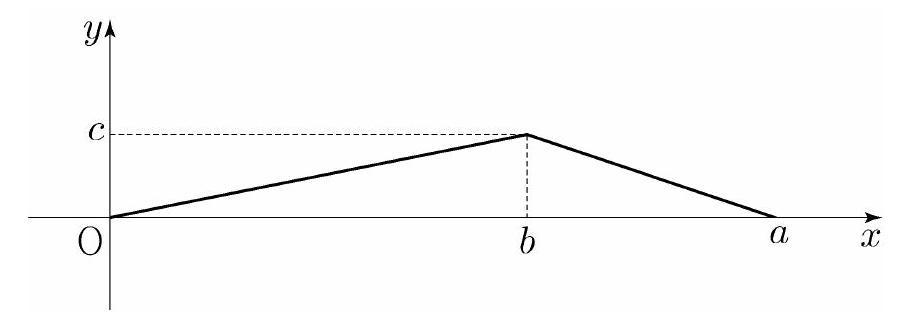
\includegraphics[max width=\textwidth]{2023_06_06_b380aa8523ec7afae994g-31}
\end{center}

$\mathrm{P}(X \leq b)-\mathrm{P}(X \geq b)=\frac{1}{4}, \mathrm{P}(X \leq \sqrt{5})=\frac{1}{2}$ 일 때, $a+b+c$ 의 값은? (단, $a, b, c$ 는 상수이다.) [4점]
(1) $\frac{11}{2}$
(2) 6
(3) $\frac{13}{2}$
(4) 7
(5) $\frac{15}{2}$

\section{4 수학 영역(확률과 통계)}
\section{단답 형}
\begin{enumerate}
  \setcounter{enumi}{28}
  \item 앞면에는 1 부터 6 까지의 자연수가 하나씩 적혀 있고 뒷면에는 모두 0 이 하나씩 적혀 있는 6 장의 카드가 있다. 이 6 장의 카드가 그림과 같이 6 이하의 자연수 $k$ 에 대하여 $k$ 번째 자리에 자연수 $k$ 가 보이도록 놓여 있다.
\end{enumerate}

\begin{center}
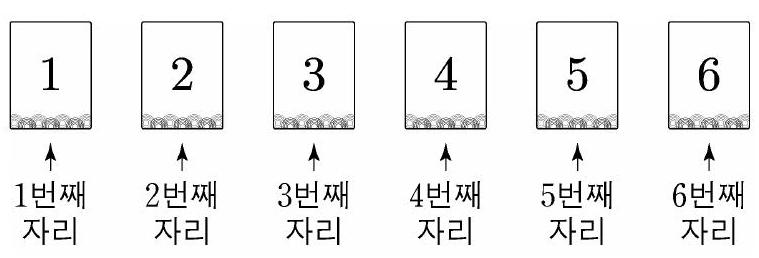
\includegraphics[max width=\textwidth]{2023_06_06_b380aa8523ec7afae994g-32}
\end{center}

이 6 장의 카드와 한 개의 주사위를 사용하여 다음 시행을 한다.

주사위를 한 번 던져 나온 눈의 수가 $k$ 이면

$k$ 번째 자리에 놓여 있는 카드를 한 번 뒤집어 제자리에 놓는다.

위의 시행을 3 번 반복한 후 6 장의 카드에 보이는 모든 수의 합이 짝수일 때, 주사위의 1 의 눈이 한 번만 나왔을 확률은 $\frac{q}{p}$ 이다. $p+q$ 의 값을 구하시오. (단, $p$ 와 $q$ 는 서로소인 자연수이다.) 30. 집합 $X=\{x \mid x$ 는 10 이하의 자연수 $\}$ 에 대하여 다음 조건을 만족시키는 함수 $f: X \rightarrow X$ 의 개수를 구하시오. [4점]

(가) 9 이하의 모든 자연수 $x$ 에 대하여 $f(x) \leq f(x+1)$ 이다.

(나) $1 \leq x \leq 5$ 일 때 $f(x) \leq x$ 이고, $6 \leq x \leq 10$ 일 때 $f(x) \geq x$ 이다.

(다) $f(6)=f(5)+6$ $*$ 확인 사항

○ 답안지의 해당란에 필요한 내용을 정확히 기입(표기)했는지 확인 하시오.

○ 이어서, 「선택과목(미적분)」 문제가 제시되오니, 자신이 선택한 과목인지 확인하시오. 제 2 교시

\section{3학년도 대학수학능력시험 문제지}
\section{수학 영역(미적분)}
짝수형

5 지선다형

\begin{enumerate}
  \setcounter{enumi}{22}
  \item $\lim _{x \rightarrow 0} \frac{\ln (x+1)}{\sqrt{x+4}-2}$ 의 값은? [2점]
(1) 1
(2) 2
(3) 3
(4) 4
(5) 5

  \item $\lim _{n \rightarrow \infty} \frac{1}{n} \sum_{k=1}^{n} \sqrt{1+\frac{3 k}{n}}$ 의 값은? [3점]
(1) $\frac{4}{3}$
(2) $\frac{13}{9}$
(3) $\frac{14}{9}$
(4) $\frac{5}{3}$
(5) $\frac{16}{9}$ 25. 등비수열 $\left\{a_{n}\right\}$ 에 대하여 $\lim _{n \rightarrow \infty} \frac{a_{n}+1}{3^{n}+2^{2 n-1}}=3$ 일 때, $a_{2}$ 의 값은? [3점]
(1) 16
(2) 18
(3) 20
(4) 22
(5) 24

  \item 그림과 같이 곡선 $y=\sqrt{\sec ^{2} x+\tan x}\left(0 \leq x \leq \frac{\pi}{3}\right)$ 와 $x$ 축, $y$ 축 및 직선 $x=\frac{\pi}{3}$ 로 둘러싸인 부분을 밑면으로 하는 입체도형이 있다. 이 입체도형을 $x$ 축에 수직인 평면으로 자른 단면이 모두 정사각형일 때, 이 입체도형의 부피는? [3점]

\end{enumerate}

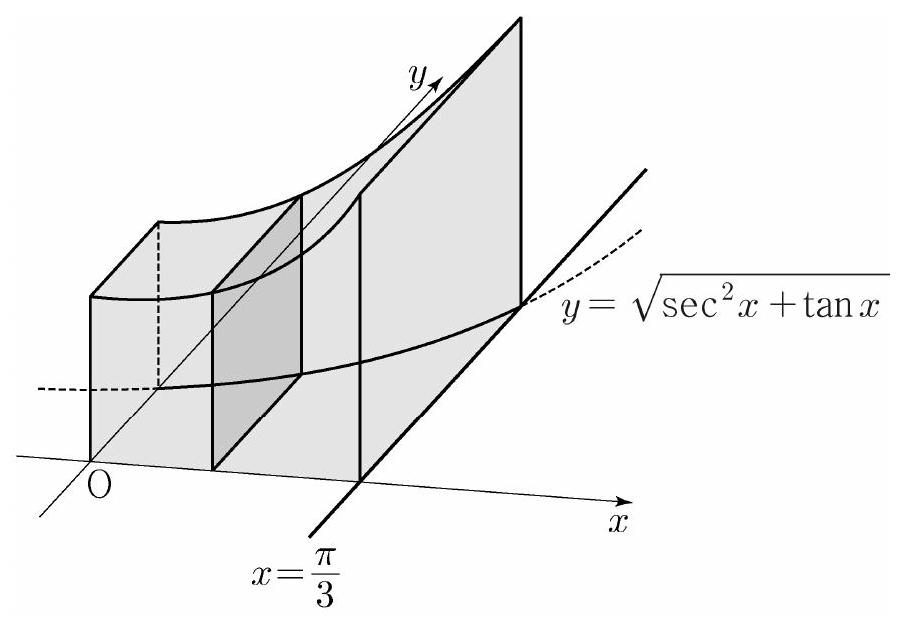
\includegraphics[max width=\textwidth, center]{2023_06_06_b380aa8523ec7afae994g-34}
(1) $\frac{\sqrt{3}}{2}+\frac{\ln 2}{2}$
(2) $\frac{\sqrt{3}}{2}+\ln 2$
(3) $\sqrt{3}+\frac{\ln 2}{2}$
(4) $\sqrt{3}+\ln 2$
(5) $\sqrt{3}+2 \ln 2$ 27. 그림과 같이 중심이 $\mathrm{O}$, 반지름의 길이가 1 이고 중심각의 크기가 $\frac{\pi}{2}$ 인 부채꼴 $\mathrm{OA}_{1} \mathrm{~B}_{1}$ 이 있다. 호 $\mathrm{A}_{1} \mathrm{~B}_{1}$ 위에 점 $\mathrm{P}_{1}$, 선분 $\mathrm{OA}_{1}$ 위에 점 $\mathrm{C}_{1}$, 선분 $\mathrm{OB}_{1}$ 위에 점 $\mathrm{D}_{1}$ 을 사각형 $\mathrm{OC}_{1} \mathrm{P}_{1} \mathrm{D}_{1}$ 이 $\overline{\mathrm{OC}_{1}}: \overline{\mathrm{OD}_{1}}=3: 4$ 인 직사각형이 되도록 잡는다. 부채꼴 $\mathrm{OA}_{1} \mathrm{~B}_{1}$ 의 내부에 점 $\mathrm{Q}_{1}$ 을 $\overline{\mathrm{P}_{1} \mathrm{Q}_{1}}=\overline{\mathrm{A}_{1} \mathrm{Q}_{1}}, \angle \mathrm{P}_{1} \mathrm{Q}_{1} \mathrm{~A}_{1}=\frac{\pi}{2}$ 가 되도록 잡고, 이등변삼각형 $\mathrm{P}_{1} \mathrm{Q}_{1} \mathrm{~A}_{1}$ 에 색칠하여 얻은 그림을 $R_{1}$ 이라 하자.

그림 $R_{1}$ 에서 선분 $\mathrm{OA}_{1}$ 위의 점 $\mathrm{A}_{2}$ 와 선분 $\mathrm{OB}_{1}$ 위의 점 $\mathrm{B}_{2}$ 를 $\overline{\mathrm{OQ}_{1}}=\overline{\mathrm{OA}_{2}}=\overline{\mathrm{OB}_{2}}$ 가 되도록 잡고, 중심이 $\mathrm{O}$, 반지름의 길이가 $\overline{\mathrm{OQ}_{1}}$, 중심각의 크기가 $\frac{\pi}{2}$ 인 부채꼴 $\mathrm{OA}_{2} \mathrm{~B}_{2}$ 를 그린다. 그림 $R_{1}$ 을 얻은 것과 같은 방법으로 네 점 $\mathrm{P}_{2}, \mathrm{C}_{2}, \mathrm{D}_{2}, \mathrm{Q}_{2}$ 를 잡고, 이등변삼각형 $\mathrm{P}_{2} \mathrm{Q}_{2} \mathrm{~A}_{2}$ 에 색칠하여 얻은 그림을 $R_{2}$ 라 하자. 이와 같은 과정을 계속하여 $n$ 번째 얻은 그림 $R_{n}$ 에 색칠되어 있는 부분의 넓이를 $S_{n}$ 이라 할 때, $\lim _{n \rightarrow \infty} S_{n}$ 의 값은? [3점]
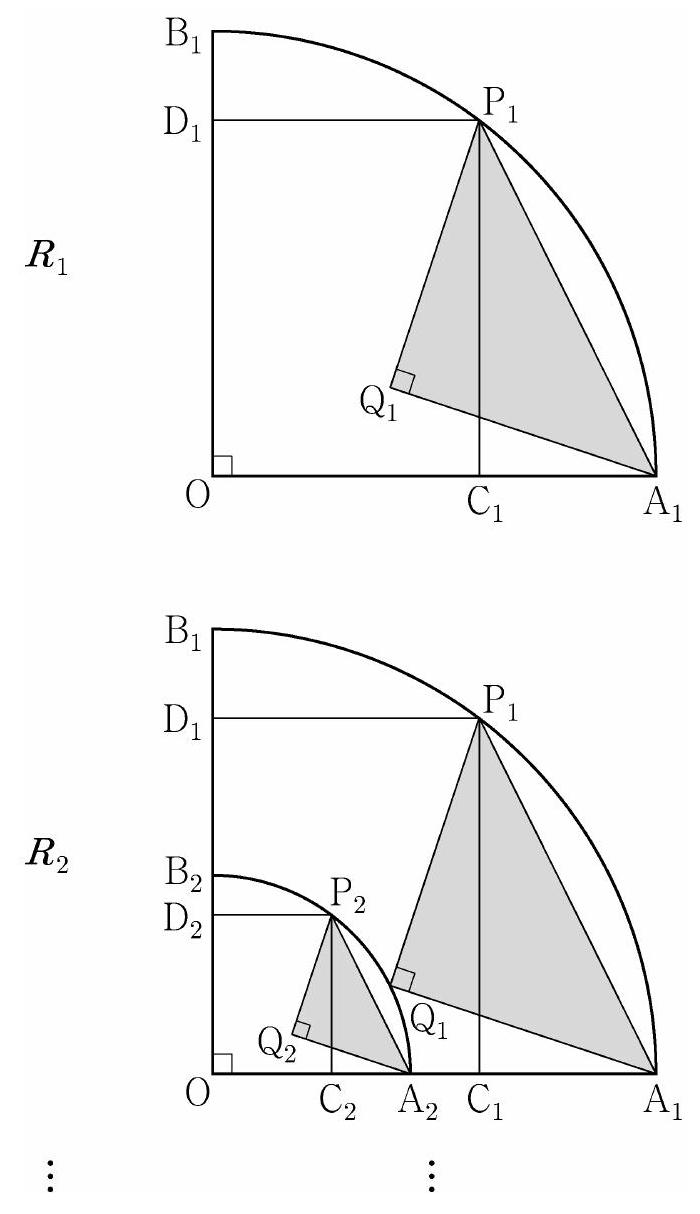
\includegraphics[max width=\textwidth, center]{2023_06_06_b380aa8523ec7afae994g-35}
(1) $\frac{9}{40}$
(2) $\frac{1}{4}$
(3) $\frac{11}{40}$
(4) $\frac{3}{10}$
(5) $\frac{13}{40}$

\begin{enumerate}
  \setcounter{enumi}{27}
  \item 그림과 같이 중심이 $\mathrm{O}$ 이고 길이가 2 인 선분 $\mathrm{AB}$ 를 지름으로 하는 반원 위에 $\angle \mathrm{AOC}=\frac{\pi}{2}$ 인 점 $\mathrm{C}$ 가 있다. 호 $\mathrm{BC}$ 위에 점 $\mathrm{P}$ 와 호 $\mathrm{CA}$ 위에 점 $\mathrm{Q}$ 를 $\overline{\mathrm{PB}}=\overline{\mathrm{QC}}$ 가 되도록 잡고, 선분 $\mathrm{AP}$ 위에 점 $\mathrm{R}$ 를 $\angle \mathrm{CQR}=\frac{\pi}{2}$ 가 되도록 잡는다. 선분 $\mathrm{AP}$ 와 선분 $\mathrm{CO}$ 의 교점을 $\mathrm{S}$ 라 하자. $\angle \mathrm{PAB}=\theta$ 일 때, 삼각형 $\mathrm{POB}$ 의 넓이를 $f(\theta)$, 사각형 $\mathrm{CQRS}$ 의 넓이를 $g(\theta)$ 라 하자. $\lim _{\theta \rightarrow 0+} \frac{3 f(\theta)-2 g(\theta)}{\theta^{2}}$ 의 값은? (단, $0<\theta<\frac{\pi}{4}$ ) [4점]
\end{enumerate}

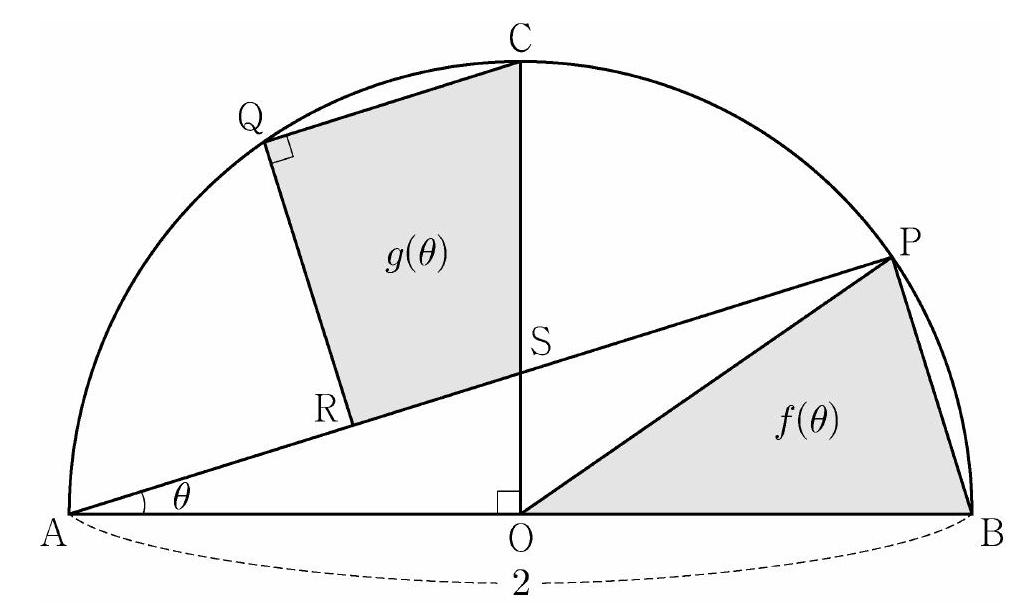
\includegraphics[max width=\textwidth, center]{2023_06_06_b380aa8523ec7afae994g-35(1)}
(1) 1
(2) 2
(3) 3
(4) 4
(5) 5

\section{4 수학 영역(미적분)}
짝수형

\section{단답형}
\begin{enumerate}
  \setcounter{enumi}{28}
  \item 세 상수 $a, b, c$ 에 대하여 함수 $f(x)=a e^{2 x}+b e^{x}+c$ 가 다음 조건을 만족시킨다.
\end{enumerate}

$$
\begin{aligned}
& \text { (가) } \lim _{x \rightarrow-\infty} \frac{f(x)+6}{e^{x}}=1 \\
& \text { (나) } f(\ln 2)=0
\end{aligned}
$$

함수 $f(x)$ 의 역함수를 $g(x)$ 라 할 때, $\int_{0}^{14} g(x) d x=p+q \ln 2$ 이다. $p+q$ 의 값을 구하시오. (단, $p, q$ 는 유리수이고, $\ln 2$ 는 무리수이다.) [4점] 30. 최고차항의 계수가 양수인 삼차함수 $f(x)$ 와 함수 $g(x)=e^{\sin \pi x}-1$ 에 대하여 실수 전체의 집합에서 정의된 합성함수 $h(x)=g(f(x))$ 가 다음 조건을 만족시킨다.

(가) 함수 $h(x)$ 는 $x=0$ 에서 극댓값 0 을 갖는다.

(나) 열린구간 $(0,3)$ 에서 방정식 $h(x)=1$ 의 서로 다른 실근의 개수는 7 이다.

$f(3)=\frac{1}{2}, f^{\prime}(3)=0$ 일 때, $f(2)=\frac{q}{p}$ 이다. $p+q$ 의 값을 구하시오. (단, $p$ 와 $q$ 는 서로소인 자연수이다.) [4점] $*$ 확인 사항

○ 답안지의 해당란에 필요한 내용을 정확히 기입(표기)했는지 확인 하시오.

○ 이어서, 「선택과목(기하)」 문제가 제시되오니, 자신이 선택한 과목인지 확인하시오. 제 2 교시

\section{3학년도 대학수학능력시험 문제지}
\section{수학 영역(기하)}
\section{짝수형}
\section{5 지선다형}
\begin{enumerate}
  \setcounter{enumi}{22}
  \item 좌표공간의 점 $\mathrm{A}(2,2,-1)$ 을 $x$ 축에 대하여 대칭이동한 점을 $\mathrm{B}$ 라 하자. 점 $\mathrm{C}(-2,1,1)$ 에 대하여 선분 $\mathrm{BC}$ 의 길이는?
\end{enumerate}

[2점]
(1) 1
(2) 2
(3) 3
(4) 4
(5) 5

\begin{enumerate}
  \setcounter{enumi}{23}
  \item 초점이 $\mathrm{F}\left(\frac{1}{3}, 0\right)$ 이고 준선이 $x=-\frac{1}{3}$ 인 포물선이 점 $(a, 2)$ 를 지날 때, $a$ 의 값은? [3점]
(1) 1
(2) 2
(3) 3
(4) 4
(5) 5 25. 타원 $\frac{x^{2}}{a^{2}}+\frac{y^{2}}{b^{2}}=1$ 위의 점 $(2,1)$ 에서의 접선의 기울기가 $-\frac{1}{2}$ 일 때, 이 타원의 두 초점 사이의 거리는? (단, $a, b$ 는 양수이다.) [3점]
(1) $2 \sqrt{3}$
(2) 4
(3) $2 \sqrt{5}$
(4) $2 \sqrt{6}$
(5) $2 \sqrt{7}$

  \item 좌표평면에서 세 벡터

\end{enumerate}

$$
\vec{a}=(2,4), \quad \vec{b}=(2,8), \quad \vec{c}=(1,0)
$$

에 대하여 두 벡터 $\vec{p}, \vec{q}$ 가

$$
(\vec{p}-\vec{a}) \cdot(\vec{p}-\vec{b})=0, \quad \vec{q}=\frac{1}{2} \vec{a}+t \vec{c}(t \text { 는 실수 })
$$

를 만족시킬 때, $|\vec{p}-\vec{q}|$ 의 최솟값은? [3점]
(1) $\frac{3}{2}$
(2) 2
(3) $\frac{5}{2}$
(4) 3
(5) $\frac{7}{2}$ 27. 좌표공간에 직선 $\mathrm{AB}$ 를 포함하는 평면 $\alpha$ 가 있다. 평면 $\alpha$ 위에 있지 않은 점 $\mathrm{C}$ 에 대하여 직선 $\mathrm{AB}$ 와 직선 $\mathrm{AC}$ 가 이루는 예각의 크기를 $\theta_{1}$ 이라 할 때 $\sin \theta_{1}=\frac{4}{5}$ 이고, 직선 $\mathrm{AC}$ 와 평면 $\alpha$ 가 이루는 예각의 크기는 $\frac{\pi}{2}-\theta_{1}$ 이다. 평면 $\mathrm{ABC}$ 와 평면 $\alpha$ 가 이루는 예각의 크기를 $\theta_{2}$ 라 할 때, $\cos \theta_{2}$ 의 값은? [3점]
(1) $\frac{\sqrt{7}}{4}$
(2) $\frac{\sqrt{7}}{5}$
(3) $\frac{\sqrt{7}}{6}$
(4) $\frac{\sqrt{7}}{7}$
(5) $\frac{\sqrt{7}}{8}$

\begin{center}
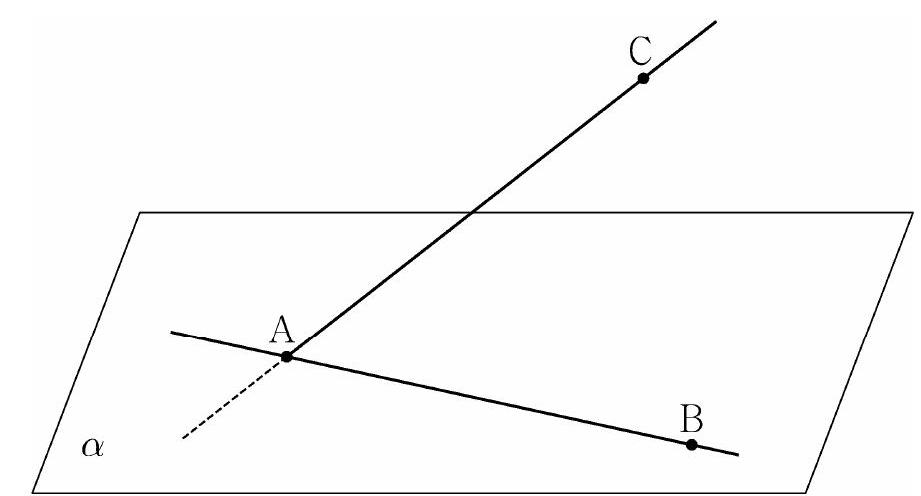
\includegraphics[max width=\textwidth]{2023_06_06_b380aa8523ec7afae994g-39(1)}
\end{center}

\begin{enumerate}
  \setcounter{enumi}{27}
  \item 두 초점이 $\mathrm{F}(c, 0), \mathrm{F}^{\prime}(-c, 0)(c>0)$ 인 쌍곡선 $C$ 와 $y$ 축 위의 점 $\mathrm{A}$ 가 있다. 쌍곡선 $C$ 가 선분 $\mathrm{AF}$ 와 만나는 점을 $\mathrm{P}$, 선분 $\mathrm{AF}^{\prime}$ 과 만나는 점을 $\mathrm{P}^{\prime}$ 이라 하자.
\end{enumerate}

직선 $\mathrm{AF}$ 는 쌍곡선 $C$ 의 한 점근선과 평행하고

$$
\overline{\mathrm{AP}}: \overline{\mathrm{PP}^{\prime}}=5: 6, \overline{\mathrm{PF}}=1
$$

일 때, 쌍곡선 $C$ 의 주축의 길이는? [4점]
(1) $\frac{13}{6}$
(2) $\frac{9}{4}$
(3) $\frac{7}{3}$
(4) $\frac{29}{12}$
(5) $\frac{5}{2}$

\begin{center}
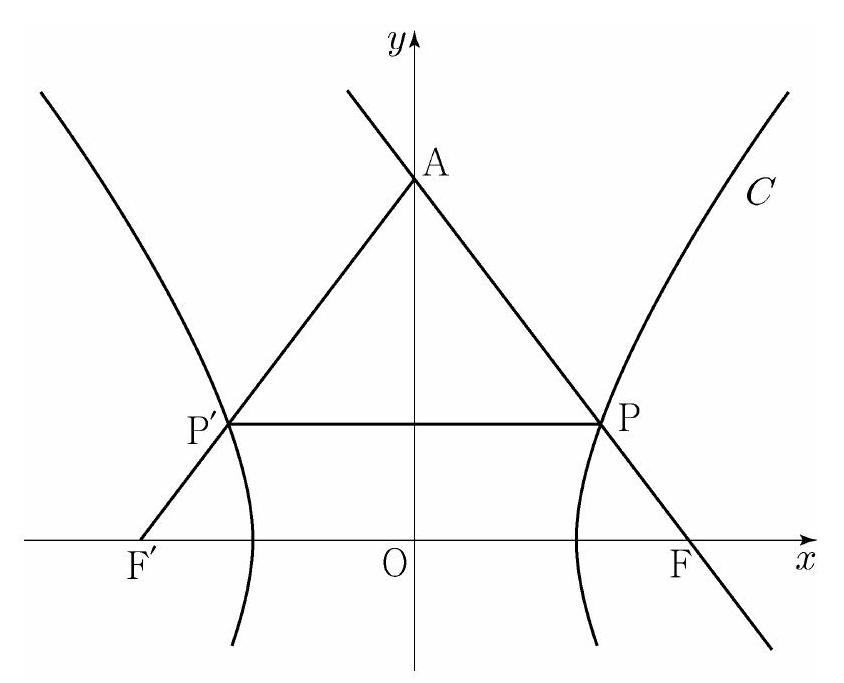
\includegraphics[max width=\textwidth]{2023_06_06_b380aa8523ec7afae994g-39}
\end{center}

\section{4 수학 영역(기하)}
짝수형

\section{단답 형}
\begin{enumerate}
  \setcounter{enumi}{28}
  \item 평면 $\alpha$ 위에 $\overline{\mathrm{AB}}=\overline{\mathrm{CD}}=\overline{\mathrm{AD}}=2, \angle \mathrm{ABC}=\angle \mathrm{BCD}=\frac{\pi}{3}$ 인 사다리꼴 $\mathrm{ABCD}$ 가 있다. 다음 조건을 만족시키는 평면 $\alpha$ 위의 두 점 $\mathrm{P}, \mathrm{Q}$ 에 대하여 $\overrightarrow{\mathrm{CP}} \cdot \overrightarrow{\mathrm{DQ}}$ 의 값을 구하시오. [4점]
(가) $\overrightarrow{\mathrm{AC}}=2(\overrightarrow{\mathrm{AD}}+\overrightarrow{\mathrm{BP}})$
(나) $\overrightarrow{\mathrm{AC}} \cdot \overrightarrow{\mathrm{PQ}}=6$
(다) $2 \times \angle \mathrm{BQA}=\angle \mathrm{PBQ}<\frac{\pi}{2}$
\end{enumerate}

\begin{center}
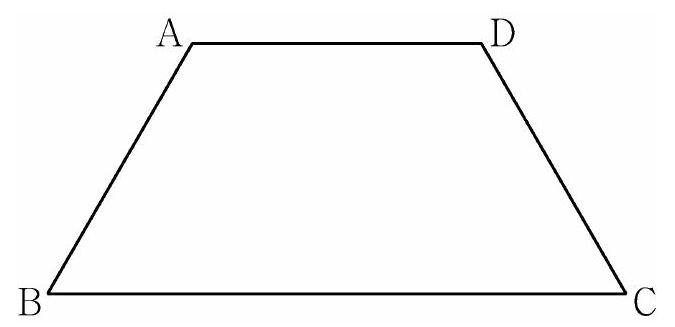
\includegraphics[max width=\textwidth]{2023_06_06_b380aa8523ec7afae994g-40(1)}
\end{center}

\begin{enumerate}
  \setcounter{enumi}{29}
  \item 좌표공간에 정사면체 $\mathrm{ABCD}$ 가 있다. 정삼각형 $\mathrm{BCD}$ 의 외심을 중심으로 하고 점 $\mathrm{B}$ 를 지나는 구를 $S$ 라 하자. 구 $S$ 와 선분 $\mathrm{AB}$ 가 만나는 점 중 $\mathrm{B}$ 가 아닌 점을 $\mathrm{P}$, 구 $S$ 와 선분 $\mathrm{AC}$ 가 만나는 점 중 $\mathrm{C}$ 가 아닌 점을 $\mathrm{Q}$, 구 $S$ 와 선분 $\mathrm{AD}$ 가 만나는 점 중 $\mathrm{D}$ 가 아닌 점을 $\mathrm{R}$ 라 하고, 점 $\mathrm{P}$ 에서 구 $S$ 에 접하는 평면을 $\alpha$ 라 하자. 구 $S$ 의 반지름의 길이가 6 일 때, 삼각형 $\mathrm{PQR}$ 의 평면 $\alpha$ 위로의 정사영의 넓이는 $k$ 이다. $k^{2}$ 의 값을 구하시오. [4점]
\end{enumerate}

\begin{center}
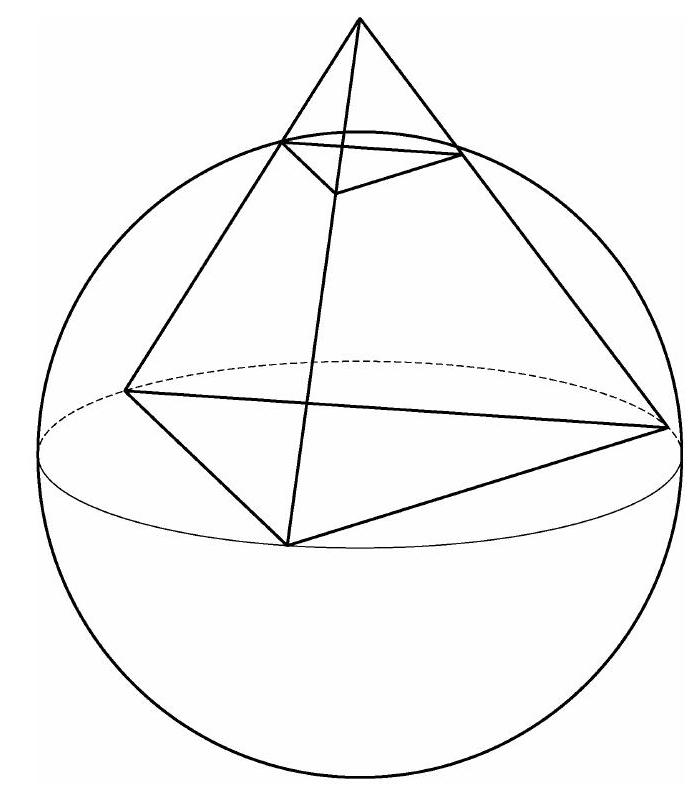
\includegraphics[max width=\textwidth]{2023_06_06_b380aa8523ec7afae994g-40}
\end{center}

\begin{itemize}
  \item 확인 사항
\end{itemize}

\begin{itemize}
  \item 답안지의 해당란에 필요한 내용을 정확히 기입(표기)했는지 확인 하시오.
\end{itemize}

\end{document}